% Options for packages loaded elsewhere
\PassOptionsToPackage{unicode}{hyperref}
\PassOptionsToPackage{hyphens}{url}
%
\documentclass[
]{article}
\title{Appendix S4}
\date{}

\usepackage{amsmath,amssymb}
\usepackage{lmodern}
\usepackage{iftex}
\ifPDFTeX
  \usepackage[T1]{fontenc}
  \usepackage[utf8]{inputenc}
  \usepackage{textcomp} % provide euro and other symbols
\else % if luatex or xetex
  \usepackage{unicode-math}
  \defaultfontfeatures{Scale=MatchLowercase}
  \defaultfontfeatures[\rmfamily]{Ligatures=TeX,Scale=1}
\fi
% Use upquote if available, for straight quotes in verbatim environments
\IfFileExists{upquote.sty}{\usepackage{upquote}}{}
\IfFileExists{microtype.sty}{% use microtype if available
  \usepackage[]{microtype}
  \UseMicrotypeSet[protrusion]{basicmath} % disable protrusion for tt fonts
}{}
\makeatletter
\@ifundefined{KOMAClassName}{% if non-KOMA class
  \IfFileExists{parskip.sty}{%
    \usepackage{parskip}
  }{% else
    \setlength{\parindent}{0pt}
    \setlength{\parskip}{6pt plus 2pt minus 1pt}}
}{% if KOMA class
  \KOMAoptions{parskip=half}}
\makeatother
\usepackage{xcolor}
\IfFileExists{xurl.sty}{\usepackage{xurl}}{} % add URL line breaks if available
\IfFileExists{bookmark.sty}{\usepackage{bookmark}}{\usepackage{hyperref}}
\hypersetup{
  pdftitle={Appendix S4},
  pdfauthor={Shelton, A.O. et al.~2022. Toward Quantitative Metabarcoding. Ecology.},
  hidelinks,
  pdfcreator={LaTeX via pandoc}}
\urlstyle{same} % disable monospaced font for URLs
\usepackage[margin=1in]{geometry}
\usepackage{color}
\usepackage{fancyvrb}
\newcommand{\VerbBar}{|}
\newcommand{\VERB}{\Verb[commandchars=\\\{\}]}
\DefineVerbatimEnvironment{Highlighting}{Verbatim}{commandchars=\\\{\}}
% Add ',fontsize=\small' for more characters per line
\usepackage{framed}
\definecolor{shadecolor}{RGB}{248,248,248}
\newenvironment{Shaded}{\begin{snugshade}}{\end{snugshade}}
\newcommand{\AlertTok}[1]{\textcolor[rgb]{0.94,0.16,0.16}{#1}}
\newcommand{\AnnotationTok}[1]{\textcolor[rgb]{0.56,0.35,0.01}{\textbf{\textit{#1}}}}
\newcommand{\AttributeTok}[1]{\textcolor[rgb]{0.77,0.63,0.00}{#1}}
\newcommand{\BaseNTok}[1]{\textcolor[rgb]{0.00,0.00,0.81}{#1}}
\newcommand{\BuiltInTok}[1]{#1}
\newcommand{\CharTok}[1]{\textcolor[rgb]{0.31,0.60,0.02}{#1}}
\newcommand{\CommentTok}[1]{\textcolor[rgb]{0.56,0.35,0.01}{\textit{#1}}}
\newcommand{\CommentVarTok}[1]{\textcolor[rgb]{0.56,0.35,0.01}{\textbf{\textit{#1}}}}
\newcommand{\ConstantTok}[1]{\textcolor[rgb]{0.00,0.00,0.00}{#1}}
\newcommand{\ControlFlowTok}[1]{\textcolor[rgb]{0.13,0.29,0.53}{\textbf{#1}}}
\newcommand{\DataTypeTok}[1]{\textcolor[rgb]{0.13,0.29,0.53}{#1}}
\newcommand{\DecValTok}[1]{\textcolor[rgb]{0.00,0.00,0.81}{#1}}
\newcommand{\DocumentationTok}[1]{\textcolor[rgb]{0.56,0.35,0.01}{\textbf{\textit{#1}}}}
\newcommand{\ErrorTok}[1]{\textcolor[rgb]{0.64,0.00,0.00}{\textbf{#1}}}
\newcommand{\ExtensionTok}[1]{#1}
\newcommand{\FloatTok}[1]{\textcolor[rgb]{0.00,0.00,0.81}{#1}}
\newcommand{\FunctionTok}[1]{\textcolor[rgb]{0.00,0.00,0.00}{#1}}
\newcommand{\ImportTok}[1]{#1}
\newcommand{\InformationTok}[1]{\textcolor[rgb]{0.56,0.35,0.01}{\textbf{\textit{#1}}}}
\newcommand{\KeywordTok}[1]{\textcolor[rgb]{0.13,0.29,0.53}{\textbf{#1}}}
\newcommand{\NormalTok}[1]{#1}
\newcommand{\OperatorTok}[1]{\textcolor[rgb]{0.81,0.36,0.00}{\textbf{#1}}}
\newcommand{\OtherTok}[1]{\textcolor[rgb]{0.56,0.35,0.01}{#1}}
\newcommand{\PreprocessorTok}[1]{\textcolor[rgb]{0.56,0.35,0.01}{\textit{#1}}}
\newcommand{\RegionMarkerTok}[1]{#1}
\newcommand{\SpecialCharTok}[1]{\textcolor[rgb]{0.00,0.00,0.00}{#1}}
\newcommand{\SpecialStringTok}[1]{\textcolor[rgb]{0.31,0.60,0.02}{#1}}
\newcommand{\StringTok}[1]{\textcolor[rgb]{0.31,0.60,0.02}{#1}}
\newcommand{\VariableTok}[1]{\textcolor[rgb]{0.00,0.00,0.00}{#1}}
\newcommand{\VerbatimStringTok}[1]{\textcolor[rgb]{0.31,0.60,0.02}{#1}}
\newcommand{\WarningTok}[1]{\textcolor[rgb]{0.56,0.35,0.01}{\textbf{\textit{#1}}}}
\usepackage{graphicx}
\makeatletter
\def\maxwidth{\ifdim\Gin@nat@width>\linewidth\linewidth\else\Gin@nat@width\fi}
\def\maxheight{\ifdim\Gin@nat@height>\textheight\textheight\else\Gin@nat@height\fi}
\makeatother
% Scale images if necessary, so that they will not overflow the page
% margins by default, and it is still possible to overwrite the defaults
% using explicit options in \includegraphics[width, height, ...]{}
\setkeys{Gin}{width=\maxwidth,height=\maxheight,keepaspectratio}
% Set default figure placement to htbp
\makeatletter
\def\fps@figure{htbp}
\makeatother
\setlength{\emergencystretch}{3em} % prevent overfull lines
\providecommand{\tightlist}{%
  \setlength{\itemsep}{0pt}\setlength{\parskip}{0pt}}
\setcounter{secnumdepth}{-\maxdimen} % remove section numbering
\usepackage{float}
\ifLuaTeX
  \usepackage{selnolig}  % disable illegal ligatures
\fi

\begin{document}
\maketitle
Shelton, A.O., Z.J. Gold, A.J. Jensen, E. D'Agnese,  E.A.
Allan, A. Van Cise, R. Gallego, A. Ramón-Laca, M. Garber-Yonts, K.
Parsons, and R.P. Kelly. 2022. Toward Quantitative Metabarcoding.  Ecology.


\subsection{Introduction}

This document accompanies ``Toward Quantitative Metabarcoding'' by
Shelton et al.~(2022) and provides a toy example for implementing the
model with empirical data. We present an example from the Pacific fish
example in the main text to illustrate implementation in practice. This
example assumes that sequencing data has been appropriately generated
and classified into taxa. Data are the number of reads associated with
each taxa in each sample.

\hypertarget{pacific-fish}{%
\subsection{Pacific Fish}\label{pacific-fish}}

This example involves using data produced by Zack Gold using mock
communities constructed from species from the California current. We use
three mock communities from the ``Ocean'' group: Ocean even, Ocean skew
1, and Ocean skew 2. There are 18 species in this set of species and as
their names suggest, Ocean even has equal abundance across all species
(5.66\% each) while the two skew communities have 4 species with
relatively high abundance (18.75\%) and 8 species with lower
contributions (3.125\% each). In the example below will use the even
communities as a known mock community and the remaining as unknown
samples.

First we need to load needed libraries and read into R the observed
sequence data.

\begin{Shaded}
\begin{Highlighting}[]
\CommentTok{\# you will need these packages to make this program run.}
\FunctionTok{library}\NormalTok{(dplyr)}
\FunctionTok{library}\NormalTok{(compositions)}
\FunctionTok{library}\NormalTok{(tidyverse)}
\FunctionTok{library}\NormalTok{(rstan)}
\FunctionTok{library}\NormalTok{(here)}
\FunctionTok{library}\NormalTok{(ggsci)}

\CommentTok{\# This is the data from Ocean communities.}
\NormalTok{dat }\OtherTok{\textless{}{-}} \FunctionTok{readRDS}\NormalTok{(}\StringTok{"Ocean\_mock\_community.RDS"}\NormalTok{)}
\CommentTok{\# Take a brief look at the data:}
\FunctionTok{head}\NormalTok{(dat)}
\end{Highlighting}
\end{Shaded}

\begin{verbatim}
## # A tibble: 6 x 6
##   ID_mifish             community      tech_rep Cycles nReads start_conc_ng
##   <chr>                 <chr>          <chr>    <chr>   <dbl>         <dbl>
## 1 Bathylagoides wesethi Oceanic_Even   1        39       4129            30
## 2 Bathylagoides wesethi Oceanic_Even   2        39       4850            30
## 3 Bathylagoides wesethi Oceanic_Even   3        39       2862            30
## 4 Bathylagoides wesethi Skew_Oceanic_1 1        39          0             0
## 5 Bathylagoides wesethi Skew_Oceanic_1 2        39          0             0
## 6 Bathylagoides wesethi Skew_Oceanic_1 3        39          0             0
\end{verbatim}

Here the columns describe the taxa (ID\_mifish), mock community
(community), technical replicate number (tech\_rep), number of PCR
cycles (Cycles), number of observed reads (nReads), and known starting
DNA concentration (start\_conc\_ng). This is the entirety of data that
is required for running the statistical model. You will note that the
starting DNA concentration is not strictly necessary; below we will
convert these starting concentrations into proportion of DNA from each
species in the mock community. These proportions will be used in the
statistical model. The data includes only the three Ocean communities
(even, skew 1, and skew 2) for a single number of PCR cycles. It
includes three technical replicates for each community.

\begin{Shaded}
\begin{Highlighting}[]
\NormalTok{dat }\SpecialCharTok{\%\textgreater{}\%} \FunctionTok{distinct}\NormalTok{(community,tech\_rep)}
\end{Highlighting}
\end{Shaded}

\begin{verbatim}
## # A tibble: 9 x 2
##   community      tech_rep
##   <chr>          <chr>   
## 1 Oceanic_Even   1       
## 2 Oceanic_Even   2       
## 3 Oceanic_Even   3       
## 4 Skew_Oceanic_1 1       
## 5 Skew_Oceanic_1 2       
## 6 Skew_Oceanic_1 3       
## 7 Skew_Oceanic_2 1       
## 8 Skew_Oceanic_2 2       
## 9 Skew_Oceanic_2 3
\end{verbatim}

and includes 18 species, each of which is present in at least one
community.

\begin{Shaded}
\begin{Highlighting}[]
\NormalTok{dat }\SpecialCharTok{\%\textgreater{}\%} \FunctionTok{distinct}\NormalTok{(ID\_mifish)}
\end{Highlighting}
\end{Shaded}

\begin{verbatim}
## # A tibble: 18 x 1
##    ID_mifish                   
##    <chr>                       
##  1 Bathylagoides wesethi       
##  2 Citharichthys sordidus      
##  3 Citharichthys stigmaeus     
##  4 Citharichthys xanthostigma  
##  5 Diogenichthys atlanticus    
##  6 Engraulis mordax            
##  7 Leuroglossus stilbius       
##  8 Lipolagus ochotensis        
##  9 Merluccius productus        
## 10 Nannobrachium ritteri       
## 11 Protomyctophum crockeri     
## 12 Sardinops sagax             
## 13 Sebastes paucispinis        
## 14 Stenobrachius leucopsarus   
## 15 Symbolophorus californiensis
## 16 Trachurus symmetricus       
## 17 Triphoturus mexicanus       
## 18 Vinciguerria lucetia
\end{verbatim}

We can make a figure showing which species occur in each sample

\begin{Shaded}
\begin{Highlighting}[]
\NormalTok{sp.by.comm.slim }\OtherTok{\textless{}{-}}\NormalTok{  dat }\SpecialCharTok{\%\textgreater{}\%}
  \FunctionTok{group\_by}\NormalTok{(}\AttributeTok{species=}\NormalTok{ID\_mifish,community) }\SpecialCharTok{\%\textgreater{}\%}
  \FunctionTok{summarise}\NormalTok{(}\AttributeTok{conc =} \FunctionTok{sum}\NormalTok{(start\_conc\_ng)) }\SpecialCharTok{\%\textgreater{}\%}
  \FunctionTok{mutate}\NormalTok{(}\AttributeTok{conc2 =} \FunctionTok{ifelse}\NormalTok{(conc}\SpecialCharTok{\textgreater{}}\DecValTok{0}\NormalTok{,}\DecValTok{1}\NormalTok{,}\DecValTok{0}\NormalTok{)) }\SpecialCharTok{\%\textgreater{}\%}
  \FunctionTok{arrange}\NormalTok{(species,community) }\SpecialCharTok{\%\textgreater{}\%} \FunctionTok{group\_by}\NormalTok{(community) }\SpecialCharTok{\%\textgreater{}\%}
  \FunctionTok{mutate}\NormalTok{(}\AttributeTok{tot\_conc =} \FunctionTok{sum}\NormalTok{(conc),}\AttributeTok{prop=}\NormalTok{conc}\SpecialCharTok{/}\NormalTok{tot\_conc) }\SpecialCharTok{\%\textgreater{}\%}
\NormalTok{  dplyr}\SpecialCharTok{::}\FunctionTok{select}\NormalTok{(}\SpecialCharTok{{-}}\NormalTok{conc,}\SpecialCharTok{{-}}\NormalTok{prop,}\SpecialCharTok{{-}}\NormalTok{tot\_conc) }\SpecialCharTok{\%\textgreater{}\%}
  \FunctionTok{pivot\_wider}\NormalTok{(}\AttributeTok{names\_from =}\NormalTok{ community,}\AttributeTok{values\_from =}\NormalTok{ conc2,}\AttributeTok{values\_fill =} \DecValTok{0}\NormalTok{) }\SpecialCharTok{\%\textgreater{}\%}
  \FunctionTok{pivot\_longer}\NormalTok{(}\SpecialCharTok{!}\NormalTok{species, }\AttributeTok{names\_to =} \StringTok{"community"}\NormalTok{,}\AttributeTok{values\_to=} \StringTok{"present"}\NormalTok{) }\SpecialCharTok{\%\textgreater{}\%} 
  \FunctionTok{mutate}\NormalTok{(}\AttributeTok{present =} \FunctionTok{as.factor}\NormalTok{(present))}

\CommentTok{\# Make some grids of species to understand overlap.}
\FunctionTok{ggplot}\NormalTok{(sp.by.comm.slim) }\SpecialCharTok{+}
  \FunctionTok{geom\_tile}\NormalTok{(}\FunctionTok{aes}\NormalTok{(}\AttributeTok{x=}\NormalTok{community,}\AttributeTok{y=}\NormalTok{species,}\AttributeTok{fill=}\NormalTok{present)) }\SpecialCharTok{+}
  \FunctionTok{scale\_fill\_viridis\_d}\NormalTok{(}\AttributeTok{option =} \StringTok{"plasma"}\NormalTok{,}\AttributeTok{end =} \FloatTok{0.75}\NormalTok{) }\SpecialCharTok{+}
  \FunctionTok{scale\_y\_discrete}\NormalTok{(}\StringTok{""}\NormalTok{) }\SpecialCharTok{+}
  \FunctionTok{theme}\NormalTok{(}\AttributeTok{axis.text.x =} \FunctionTok{element\_text}\NormalTok{(}\AttributeTok{angle=}\DecValTok{90}\NormalTok{) ) }
\end{Highlighting}
\end{Shaded}

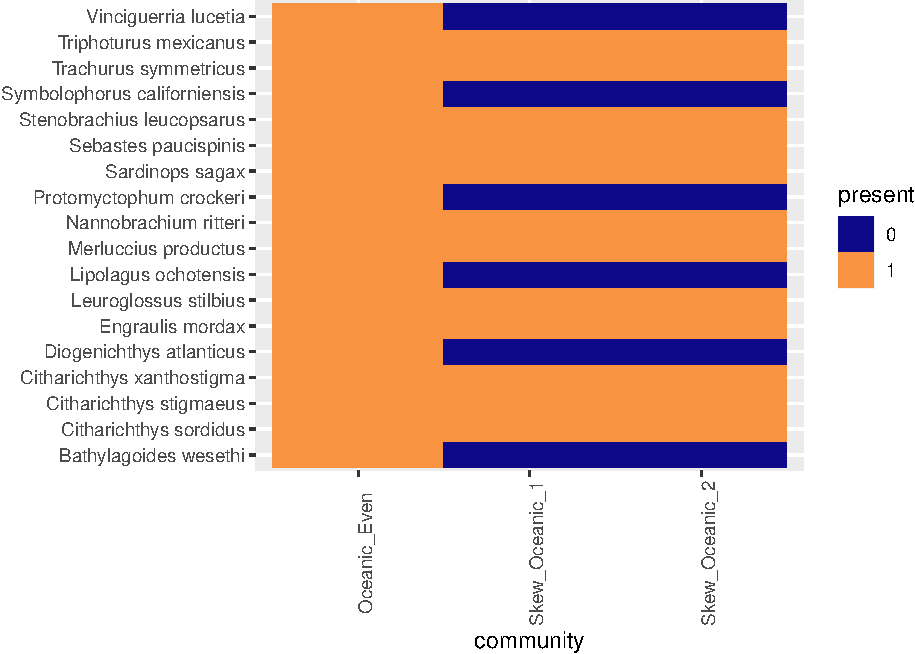
\includegraphics{Appendix-S4_files/figure-latex/which_sp-1.pdf}

\hypertarget{setting-up-data-frames-for-analysis}{%
\subsection{Setting up data frames for
analysis}\label{setting-up-data-frames-for-analysis}}

As in the main text of the manuscript, we will treat the skew
communities as field samples of unknown composition and the even
community as the mock community of known composition.

\begin{Shaded}
\begin{Highlighting}[]
\CommentTok{\#set up environmental/unknown samples}
\NormalTok{  env }\OtherTok{\textless{}{-}}\NormalTok{ dat }\SpecialCharTok{\%\textgreater{}\%}  
            \FunctionTok{rename}\NormalTok{(}\StringTok{"Species"} \OtherTok{=} \StringTok{"ID\_mifish"}\NormalTok{) }\SpecialCharTok{\%\textgreater{}\%} 
            \FunctionTok{group\_by}\NormalTok{(community,tech\_rep) }\SpecialCharTok{\%\textgreater{}\%} 
            \FunctionTok{mutate}\NormalTok{(}\AttributeTok{propReads =}\NormalTok{ nReads}\SpecialCharTok{/}\FunctionTok{sum}\NormalTok{(nReads), }\CommentTok{\#calculate proportion of reads}
                 \AttributeTok{totReads =} \FunctionTok{sum}\NormalTok{(nReads)) }\SpecialCharTok{\%\textgreater{}\%}  \CommentTok{\#calculate total reads for community}
            \FunctionTok{group\_by}\NormalTok{(Species) }\SpecialCharTok{\%\textgreater{}\%} 
            \FunctionTok{mutate}\NormalTok{(}\AttributeTok{totalSpeciesReads =} \FunctionTok{sum}\NormalTok{(nReads)) }\SpecialCharTok{\%\textgreater{}\%}  
            \FunctionTok{add\_tally}\NormalTok{(nReads }\SpecialCharTok{\textgreater{}} \DecValTok{0}\NormalTok{, }\AttributeTok{name =} \StringTok{"totalOccurrences"}\NormalTok{) }\SpecialCharTok{\%\textgreater{}\%} 
            \FunctionTok{filter}\NormalTok{(totalSpeciesReads }\SpecialCharTok{\textgreater{}} \DecValTok{0}\NormalTok{) }
    
  \CommentTok{\#assign most common species in the observed sequences to be the reference species}
\NormalTok{  mostCommon }\OtherTok{\textless{}{-}}\NormalTok{ env }\SpecialCharTok{\%\textgreater{}\%} 
    \FunctionTok{group\_by}\NormalTok{(Species) }\SpecialCharTok{\%\textgreater{}\%} 
    \FunctionTok{tally}\NormalTok{(nReads }\SpecialCharTok{\textgreater{}} \DecValTok{0}\NormalTok{) }\SpecialCharTok{\%\textgreater{}\%}
    \FunctionTok{arrange}\NormalTok{(}\FunctionTok{desc}\NormalTok{(n)) }\SpecialCharTok{\%\textgreater{}\%} 
    \FunctionTok{head}\NormalTok{(}\DecValTok{1}\NormalTok{) }\SpecialCharTok{\%\textgreater{}\%} 
    \FunctionTok{pull}\NormalTok{(Species)}
  \CommentTok{\#make the most common species the reference species}
\NormalTok{  env}\SpecialCharTok{$}\NormalTok{Species[env}\SpecialCharTok{$}\NormalTok{Species }\SpecialCharTok{==}\NormalTok{ mostCommon] }\OtherTok{\textless{}{-}} \FunctionTok{paste0}\NormalTok{(}\StringTok{"zRefSpecies\_"}\NormalTok{, mostCommon) }
\NormalTok{  env }\OtherTok{\textless{}{-}}\NormalTok{ env }\SpecialCharTok{\%\textgreater{}\%} 
    \FunctionTok{arrange}\NormalTok{(Species, community)}

\CommentTok{\# set up mock communities}
\NormalTok{  mc }\OtherTok{\textless{}{-}}\NormalTok{ dat }\SpecialCharTok{\%\textgreater{}\%}  
    \FunctionTok{filter}\NormalTok{(}\FunctionTok{str\_detect}\NormalTok{(community, }\StringTok{"Even"}\NormalTok{)) }\SpecialCharTok{\%\textgreater{}\%}
    \FunctionTok{rename}\NormalTok{(}\StringTok{"Species"} \OtherTok{=} \StringTok{"ID\_mifish"}\NormalTok{)  }\CommentTok{\#mock comm samples}
  \CommentTok{\#make the most common species the reference species}
\NormalTok{    mc}\SpecialCharTok{$}\NormalTok{Species[mc}\SpecialCharTok{$}\NormalTok{Species }\SpecialCharTok{==}\NormalTok{ mostCommon] }\OtherTok{\textless{}{-}} \FunctionTok{paste0}\NormalTok{(}\StringTok{"zRefSpecies\_"}\NormalTok{, mostCommon)   }
  
  \CommentTok{\# Filter so that you only keep species in the environment samples that are in the mock community.}
  \CommentTok{\# It is ok to include species that are only in the mock community.}
\NormalTok{  env }\OtherTok{\textless{}{-}}\NormalTok{ env }\SpecialCharTok{\%\textgreater{}\%}
      \FunctionTok{filter}\NormalTok{(}\FunctionTok{str\_detect}\NormalTok{(community, }\StringTok{"Even"}\NormalTok{,}\AttributeTok{negate =} \ConstantTok{TRUE}\NormalTok{)) }\SpecialCharTok{\%\textgreater{}\%}
      \FunctionTok{filter}\NormalTok{(Species }\SpecialCharTok{\%in\%}\NormalTok{ mc}\SpecialCharTok{$}\NormalTok{Species)}\SpecialCharTok{\%\textgreater{}\%} \CommentTok{\#limit to species occurring in mock community dataset}
      \FunctionTok{arrange}\NormalTok{(Species, community)  }
  
  \CommentTok{\#double check}
  \FunctionTok{sum}\NormalTok{(}\SpecialCharTok{!}\NormalTok{mc}\SpecialCharTok{$}\NormalTok{Species }\SpecialCharTok{\%in\%} \FunctionTok{unique}\NormalTok{(env}\SpecialCharTok{$}\NormalTok{Species)) }\CommentTok{\# This can be non{-}zero}
\end{Highlighting}
\end{Shaded}

\begin{verbatim}
## [1] 0
\end{verbatim}

\begin{Shaded}
\begin{Highlighting}[]
  \FunctionTok{sum}\NormalTok{(}\SpecialCharTok{!}\NormalTok{env}\SpecialCharTok{$}\NormalTok{Species }\SpecialCharTok{\%in\%} \FunctionTok{unique}\NormalTok{(mc}\SpecialCharTok{$}\NormalTok{Species)) }\CommentTok{\# this had better be zero.}
\end{Highlighting}
\end{Shaded}

\begin{verbatim}
## [1] 0
\end{verbatim}

\begin{Shaded}
\begin{Highlighting}[]
  \CommentTok{\# Make a single species list:}
\NormalTok{    sp.list   }\OtherTok{\textless{}{-}} \FunctionTok{data.frame}\NormalTok{(}\AttributeTok{Species =} \FunctionTok{sort}\NormalTok{(}\FunctionTok{unique}\NormalTok{(mc}\SpecialCharTok{$}\NormalTok{Species))) }\SpecialCharTok{\%\textgreater{}\%} \FunctionTok{mutate}\NormalTok{(}\AttributeTok{sp\_idx =}\DecValTok{1}\SpecialCharTok{:}\FunctionTok{length}\NormalTok{(Species))}
\NormalTok{    N\_species }\OtherTok{\textless{}{-}} \FunctionTok{nrow}\NormalTok{(sp.list)}
    
\NormalTok{    comm.mock.list }\OtherTok{\textless{}{-}}\NormalTok{ mc }\SpecialCharTok{\%\textgreater{}\%} \FunctionTok{group\_by}\NormalTok{(community, tech\_rep,Cycles) }\SpecialCharTok{\%\textgreater{}\%} 
                        \FunctionTok{summarise}\NormalTok{(}\AttributeTok{n=}\FunctionTok{length}\NormalTok{(tech\_rep)) }\SpecialCharTok{\%\textgreater{}\%}
                        \FunctionTok{ungroup}\NormalTok{() }\SpecialCharTok{\%\textgreater{}\%} 
                        \FunctionTok{mutate}\NormalTok{(}\AttributeTok{id=}\DecValTok{1}\SpecialCharTok{:}\FunctionTok{length}\NormalTok{(n))}
\NormalTok{    comm.env.list   }\OtherTok{\textless{}{-}}\NormalTok{ env }\SpecialCharTok{\%\textgreater{}\%} \FunctionTok{group\_by}\NormalTok{(community, tech\_rep,Cycles) }\SpecialCharTok{\%\textgreater{}\%} 
                        \FunctionTok{summarise}\NormalTok{(}\AttributeTok{n=}\FunctionTok{length}\NormalTok{(tech\_rep)) }\SpecialCharTok{\%\textgreater{}\%}
                        \FunctionTok{ungroup}\NormalTok{() }\SpecialCharTok{\%\textgreater{}\%} \FunctionTok{mutate}\NormalTok{(}\AttributeTok{id=}\DecValTok{1}\SpecialCharTok{:}\FunctionTok{length}\NormalTok{(n))}
    
    \CommentTok{\#make a list of species that are in mock community but not environment, }
    \CommentTok{\# expand grid to make it so the the environmental samples get padded with all the}
    \CommentTok{\# missing species for all of the communities and all tech replicates.}
    
\NormalTok{    sp.comm.mc  }\OtherTok{\textless{}{-}} \FunctionTok{expand\_grid}\NormalTok{(}\AttributeTok{Species =}\NormalTok{ sp.list}\SpecialCharTok{$}\NormalTok{Species, }\AttributeTok{id =}\NormalTok{ comm.mock.list}\SpecialCharTok{$}\NormalTok{id) }\SpecialCharTok{\%\textgreater{}\%} 
                          \FunctionTok{left\_join}\NormalTok{(.,sp.list }\SpecialCharTok{\%\textgreater{}\%}\NormalTok{ dplyr}\SpecialCharTok{::}\FunctionTok{select}\NormalTok{(Species,sp\_idx)) }\SpecialCharTok{\%\textgreater{}\%}
                          \FunctionTok{left\_join}\NormalTok{(.,comm.mock.list }\SpecialCharTok{\%\textgreater{}\%} 
\NormalTok{                          dplyr}\SpecialCharTok{::}\FunctionTok{select}\NormalTok{(community,tech\_rep,Cycles,id) ) }\SpecialCharTok{\%\textgreater{}\%}
\NormalTok{                          dplyr}\SpecialCharTok{::}\FunctionTok{select}\NormalTok{(}\SpecialCharTok{{-}}\NormalTok{id)}
\NormalTok{    sp.comm.env }\OtherTok{\textless{}{-}} \FunctionTok{expand\_grid}\NormalTok{(}\AttributeTok{Species =}\NormalTok{ sp.list}\SpecialCharTok{$}\NormalTok{Species, }\AttributeTok{id =}\NormalTok{ comm.env.list}\SpecialCharTok{$}\NormalTok{id) }\SpecialCharTok{\%\textgreater{}\%} 
                          \FunctionTok{left\_join}\NormalTok{(.,sp.list }\SpecialCharTok{\%\textgreater{}\%}\NormalTok{ dplyr}\SpecialCharTok{::}\FunctionTok{select}\NormalTok{(Species,sp\_idx)) }\SpecialCharTok{\%\textgreater{}\%}
                          \FunctionTok{left\_join}\NormalTok{(.,comm.env.list }\SpecialCharTok{\%\textgreater{}\%} 
\NormalTok{                          dplyr}\SpecialCharTok{::}\FunctionTok{select}\NormalTok{(community,tech\_rep,Cycles,id) ) }\SpecialCharTok{\%\textgreater{}\%}
\NormalTok{                          dplyr}\SpecialCharTok{::}\FunctionTok{select}\NormalTok{(}\SpecialCharTok{{-}}\NormalTok{id)}

    \CommentTok{\# convert data from long{-}form to wide{-}form}
    \CommentTok{\# merge in species and indices first to make pivoting more efficient.}
\NormalTok{    mc  }\OtherTok{\textless{}{-}} \FunctionTok{left\_join}\NormalTok{(sp.comm.mc,mc) }\SpecialCharTok{\%\textgreater{}\%}
              \FunctionTok{mutate}\NormalTok{(}\AttributeTok{nReads =} \FunctionTok{ifelse}\NormalTok{(}\FunctionTok{is.na}\NormalTok{(nReads),}\DecValTok{0}\NormalTok{,nReads),}
              \AttributeTok{start\_conc\_ng =} \FunctionTok{ifelse}\NormalTok{(}\FunctionTok{is.na}\NormalTok{(start\_conc\_ng),}\DecValTok{0}\NormalTok{,start\_conc\_ng)) }
\NormalTok{    env }\OtherTok{\textless{}{-}} \FunctionTok{left\_join}\NormalTok{(sp.comm.env,env) }\SpecialCharTok{\%\textgreater{}\%}
              \FunctionTok{mutate}\NormalTok{(}\AttributeTok{nReads =} \FunctionTok{ifelse}\NormalTok{(}\FunctionTok{is.na}\NormalTok{(nReads),}\DecValTok{0}\NormalTok{,nReads),}
              \AttributeTok{start\_conc\_ng =} \FunctionTok{ifelse}\NormalTok{(}\FunctionTok{is.na}\NormalTok{(start\_conc\_ng),}\DecValTok{0}\NormalTok{,start\_conc\_ng)) }
    
    \CommentTok{\# this will be the unknown sample data}
\NormalTok{    sample\_data }\OtherTok{\textless{}{-}}\NormalTok{ env }\SpecialCharTok{\%\textgreater{}\%} 
      \FunctionTok{ungroup}\NormalTok{() }\SpecialCharTok{\%\textgreater{}\%} 
\NormalTok{      dplyr}\SpecialCharTok{::}\FunctionTok{select}\NormalTok{(community, sp\_idx, nReads,tech\_rep, Cycles) }\SpecialCharTok{\%\textgreater{}\%} 
      \FunctionTok{arrange}\NormalTok{(sp\_idx) }\SpecialCharTok{\%\textgreater{}\%} 
      \FunctionTok{pivot\_wider}\NormalTok{(}\AttributeTok{names\_from =} \StringTok{"sp\_idx"}\NormalTok{, }\AttributeTok{values\_from =} \StringTok{"nReads"}\NormalTok{, }\AttributeTok{values\_fill =} \DecValTok{0}\NormalTok{) }\SpecialCharTok{\%\textgreater{}\%}
      \FunctionTok{mutate}\NormalTok{(}\AttributeTok{Cycles =} \FunctionTok{as.numeric}\NormalTok{(Cycles))}
    
    \CommentTok{\# Make a simple data structure that will only be used for make posterior predictions }
\NormalTok{    sample\_data\_small }\OtherTok{\textless{}{-}}\NormalTok{ sample\_data }\SpecialCharTok{\%\textgreater{}\%} \FunctionTok{filter}\NormalTok{(tech\_rep}\SpecialCharTok{==}\DecValTok{1}\NormalTok{)}
    
    \CommentTok{\# this will be the mock community sample data}
\NormalTok{    mock\_data }\OtherTok{\textless{}{-}}\NormalTok{ mc }\SpecialCharTok{\%\textgreater{}\%} 
      \FunctionTok{ungroup}\NormalTok{() }\SpecialCharTok{\%\textgreater{}\%} 
\NormalTok{      dplyr}\SpecialCharTok{::}\FunctionTok{select}\NormalTok{(community, sp\_idx, nReads,tech\_rep, Cycles) }\SpecialCharTok{\%\textgreater{}\%} 
      \FunctionTok{arrange}\NormalTok{(sp\_idx) }\SpecialCharTok{\%\textgreater{}\%} 
      \FunctionTok{pivot\_wider}\NormalTok{(}\AttributeTok{names\_from =} \StringTok{"sp\_idx"}\NormalTok{, }\AttributeTok{values\_from =} \StringTok{"nReads"}\NormalTok{, }\AttributeTok{values\_fill =} \DecValTok{0}\NormalTok{) }\SpecialCharTok{\%\textgreater{}\%}
      \FunctionTok{mutate}\NormalTok{(}\AttributeTok{Cycles =} \FunctionTok{as.numeric}\NormalTok{(Cycles))}

\NormalTok{    mock\_data\_small }\OtherTok{\textless{}{-}}\NormalTok{ mock\_data }\SpecialCharTok{\%\textgreater{}\%} \FunctionTok{filter}\NormalTok{(tech\_rep}\SpecialCharTok{==}\DecValTok{1}\NormalTok{)}

\CommentTok{\#proportions}
\NormalTok{p\_mock }\OtherTok{\textless{}{-}}\NormalTok{ mc }\SpecialCharTok{\%\textgreater{}\%} 
  \FunctionTok{select}\NormalTok{(community, tech\_rep, sp\_idx, start\_conc\_ng, Cycles) }\SpecialCharTok{\%\textgreater{}\%} 
  \FunctionTok{arrange}\NormalTok{(sp\_idx) }\SpecialCharTok{\%\textgreater{}\%} 
  \FunctionTok{group\_by}\NormalTok{(community, tech\_rep, Cycles) }\SpecialCharTok{\%\textgreater{}\%} 
  \FunctionTok{mutate}\NormalTok{(}\AttributeTok{prop\_conc =}\NormalTok{ start\_conc\_ng}\SpecialCharTok{/}\FunctionTok{sum}\NormalTok{(start\_conc\_ng)) }\SpecialCharTok{\%\textgreater{}\%} 
  \FunctionTok{select}\NormalTok{(}\SpecialCharTok{{-}}\NormalTok{start\_conc\_ng) }\SpecialCharTok{\%\textgreater{}\%} \CommentTok{\#, {-}Species) \%\textgreater{}\% }
  \FunctionTok{pivot\_wider}\NormalTok{(}\AttributeTok{names\_from =} \StringTok{"sp\_idx"}\NormalTok{, }\AttributeTok{values\_from =} \StringTok{"prop\_conc"}\NormalTok{, }\AttributeTok{values\_fill =} \DecValTok{0}\NormalTok{) }\SpecialCharTok{\%\textgreater{}\%} 
  \FunctionTok{ungroup}\NormalTok{() }\SpecialCharTok{\%\textgreater{}\%} 
  \FunctionTok{arrange}\NormalTok{(community)}
  \CommentTok{\#select({-}community)}

\NormalTok{p\_mock\_small }\OtherTok{\textless{}{-}}\NormalTok{ mc }\SpecialCharTok{\%\textgreater{}\%} 
  \FunctionTok{filter}\NormalTok{(tech\_rep }\SpecialCharTok{==} \DecValTok{1}\NormalTok{) }\SpecialCharTok{\%\textgreater{}\%} 
  \FunctionTok{select}\NormalTok{(community, sp\_idx, start\_conc\_ng, Cycles) }\SpecialCharTok{\%\textgreater{}\%} 
  \FunctionTok{arrange}\NormalTok{(sp\_idx) }\SpecialCharTok{\%\textgreater{}\%} 
  \FunctionTok{group\_by}\NormalTok{(community) }\SpecialCharTok{\%\textgreater{}\%} 
  \FunctionTok{mutate}\NormalTok{(}\AttributeTok{prop\_conc =}\NormalTok{ start\_conc\_ng}\SpecialCharTok{/}\FunctionTok{sum}\NormalTok{(start\_conc\_ng)) }\SpecialCharTok{\%\textgreater{}\%} 
  \FunctionTok{select}\NormalTok{(}\SpecialCharTok{{-}}\NormalTok{start\_conc\_ng) }\SpecialCharTok{\%\textgreater{}\%}  \CommentTok{\# {-}Species) \%\textgreater{}\% }
  \FunctionTok{pivot\_wider}\NormalTok{(}\AttributeTok{names\_from =} \StringTok{"sp\_idx"}\NormalTok{, }\AttributeTok{values\_from =} \StringTok{"prop\_conc"}\NormalTok{, }\AttributeTok{values\_fill =} \DecValTok{0}\NormalTok{) }\SpecialCharTok{\%\textgreater{}\%} 
  \FunctionTok{ungroup}\NormalTok{() }\SpecialCharTok{\%\textgreater{}\%} 
  \FunctionTok{arrange}\NormalTok{(community)}
  \CommentTok{\#select({-}community, {-}Cycles)}

  \CommentTok{\#calculate additive log ratios}
  \CommentTok{\# this means reference species is 0 and all other species are relative to that species.}
  \CommentTok{\# add a trivial amount of proportion to each species (1e{-}12) to avoid logarithms of zero.}
\NormalTok{  alr\_mock\_true\_prop }\OtherTok{\textless{}{-}}\NormalTok{ p\_mock[,}\DecValTok{4}\SpecialCharTok{:}\NormalTok{(}\FunctionTok{ncol}\NormalTok{(p\_mock)}\SpecialCharTok{{-}}\DecValTok{1}\NormalTok{)]}\SpecialCharTok{*}\DecValTok{0}
  \ControlFlowTok{for}\NormalTok{(i }\ControlFlowTok{in} \DecValTok{1}\SpecialCharTok{:}\FunctionTok{nrow}\NormalTok{(p\_mock))\{}
\NormalTok{    alr\_mock\_true\_prop[i,] }\OtherTok{\textless{}{-}} \FunctionTok{alr}\NormalTok{(p\_mock[i,}\DecValTok{4}\SpecialCharTok{:}\NormalTok{(}\FunctionTok{ncol}\NormalTok{(p\_mock))] }\SpecialCharTok{+} \FloatTok{1e{-}12}\NormalTok{)}
\NormalTok{  \}}
\NormalTok{  alr\_mock\_true\_prop[,N\_species] }\OtherTok{\textless{}{-}} \DecValTok{0} \CommentTok{\#adding explicit reference species column}
  
\NormalTok{  alr\_mock\_true\_prop\_small }\OtherTok{\textless{}{-}}\NormalTok{ p\_mock\_small[,}\DecValTok{3}\SpecialCharTok{:}\NormalTok{(}\FunctionTok{ncol}\NormalTok{(p\_mock\_small)}\SpecialCharTok{{-}}\DecValTok{1}\NormalTok{)]}\SpecialCharTok{*}\DecValTok{0}
  \ControlFlowTok{for}\NormalTok{(i }\ControlFlowTok{in} \DecValTok{1}\SpecialCharTok{:}\FunctionTok{nrow}\NormalTok{(p\_mock\_small))\{}
\NormalTok{    alr\_mock\_true\_prop\_small[i,] }\OtherTok{\textless{}{-}} \FunctionTok{alr}\NormalTok{(p\_mock\_small[i,}\DecValTok{3}\SpecialCharTok{:}\NormalTok{(}\FunctionTok{ncol}\NormalTok{(p\_mock\_small))] }\SpecialCharTok{+} \FloatTok{1e{-}12}\NormalTok{)}
\NormalTok{  \}}
\NormalTok{  alr\_mock\_true\_prop\_small[,N\_species] }\OtherTok{\textless{}{-}} \DecValTok{0} 
\end{Highlighting}
\end{Shaded}

\hypertarget{create-design-matrices-for-fitting-the-model}{%
\subsection{Create design matrices for fitting the
model}\label{create-design-matrices-for-fitting-the-model}}

This section mostly makes matrices that are useful for performing matrix
multiplication in the estimation model.

\begin{Shaded}
\begin{Highlighting}[]
\CommentTok{\# Make DESIGN MATRICES for the betas (site{-}specific relative abundance)}
\CommentTok{\# and the alphas (amplification efficiencies) }

  \DocumentationTok{\#\#\#\#\# Mock communities first}
  \CommentTok{\# Make a vector of PCR cycles.}
\NormalTok{  N\_pcr\_mock }\OtherTok{\textless{}{-}}\NormalTok{ mock\_data}\SpecialCharTok{$}\NormalTok{Cycles}
  
  \CommentTok{\# For the mock communities, you only need the relative amplification efficiencies. }
  \CommentTok{\# efficiencies (alphas)}
\NormalTok{  formula\_a }\OtherTok{\textless{}{-}}\NormalTok{ community }\SpecialCharTok{\textasciitilde{}}\NormalTok{ Cycles }\SpecialCharTok{{-}}\DecValTok{1}
\NormalTok{  model\_frame }\OtherTok{\textless{}{-}} \FunctionTok{model.frame}\NormalTok{(formula\_a, mock\_data)}
\NormalTok{  model\_vector\_a\_mock }\OtherTok{\textless{}{-}} \FunctionTok{model.matrix}\NormalTok{(formula\_a, model\_frame) }\SpecialCharTok{\%\textgreater{}\%} \FunctionTok{as.numeric}\NormalTok{()}
  
\NormalTok{  N\_obs\_mock       }\OtherTok{\textless{}{-}} \FunctionTok{nrow}\NormalTok{(mock\_data)}
  \CommentTok{\# For the unknown communities, you need to make a design matrix for the sites (betas)}
  \CommentTok{\# and second component for the amplification efficiencies.}
  
  \CommentTok{\# use sample\_data}
\NormalTok{  N\_pcr\_samp }\OtherTok{\textless{}{-}}\NormalTok{ sample\_data}\SpecialCharTok{$}\NormalTok{Cycles}
  
  \ControlFlowTok{if}\NormalTok{(}\FunctionTok{length}\NormalTok{(}\FunctionTok{unique}\NormalTok{(sample\_data}\SpecialCharTok{$}\NormalTok{community))}\SpecialCharTok{==}\DecValTok{1}\NormalTok{)\{}
\NormalTok{    formula\_b }\OtherTok{\textless{}{-}}\NormalTok{ Cycles }\SpecialCharTok{\textasciitilde{}} \DecValTok{1}  
\NormalTok{  \} }\ControlFlowTok{else}\NormalTok{ \{}
\NormalTok{    formula\_b }\OtherTok{\textless{}{-}}\NormalTok{ Cycles }\SpecialCharTok{\textasciitilde{}}\NormalTok{ community}
\NormalTok{  \}}
\NormalTok{  model\_frame }\OtherTok{\textless{}{-}} \FunctionTok{model.frame}\NormalTok{(formula\_b, sample\_data)}
\NormalTok{  model\_matrix\_b\_samp }\OtherTok{\textless{}{-}} \FunctionTok{model.matrix}\NormalTok{(formula\_b, model\_frame)}
  
  \CommentTok{\# This is a model frame for making a single prediction for each site.}
\NormalTok{  model\_frame }\OtherTok{\textless{}{-}} \FunctionTok{model.frame}\NormalTok{(formula\_b, sample\_data\_small)}
\NormalTok{  model\_matrix\_b\_samp\_small }\OtherTok{\textless{}{-}} \FunctionTok{model.matrix}\NormalTok{(formula\_b, model\_frame)}
  
  \CommentTok{\# efficiencies (alphas)}
  \CommentTok{\# for all observations}
\NormalTok{  formula\_a }\OtherTok{\textless{}{-}}\NormalTok{ community }\SpecialCharTok{\textasciitilde{}}\NormalTok{ Cycles }\SpecialCharTok{{-}}\DecValTok{1}
\NormalTok{  model\_frame }\OtherTok{\textless{}{-}} \FunctionTok{model.frame}\NormalTok{(formula\_a, sample\_data)}
\NormalTok{  model\_vector\_a\_samp }\OtherTok{\textless{}{-}} \FunctionTok{model.matrix}\NormalTok{(formula\_a, model\_frame) }\SpecialCharTok{\%\textgreater{}\%} \FunctionTok{as.numeric}\NormalTok{()}
  \CommentTok{\# for a single observation for each site}
\NormalTok{  model\_frame }\OtherTok{\textless{}{-}} \FunctionTok{model.frame}\NormalTok{(formula\_a, sample\_data\_small)}
\NormalTok{  model\_vector\_a\_samp\_small }\OtherTok{\textless{}{-}} \FunctionTok{model.matrix}\NormalTok{(formula\_a, model\_frame) }\SpecialCharTok{\%\textgreater{}\%} \FunctionTok{as.numeric}\NormalTok{()}
  
  \CommentTok{\#counters }
\NormalTok{  N\_obs\_samp\_small }\OtherTok{\textless{}{-}} \FunctionTok{nrow}\NormalTok{(model\_matrix\_b\_samp\_small)}
\NormalTok{  N\_obs\_samp }\OtherTok{\textless{}{-}} \FunctionTok{nrow}\NormalTok{(sample\_data)}
\NormalTok{  N\_b\_samp\_col }\OtherTok{\textless{}{-}} \FunctionTok{ncol}\NormalTok{(model\_matrix\_b\_samp)  }
\end{Highlighting}
\end{Shaded}

\hypertarget{model-estimation}{%
\subsection{Model estimation}\label{model-estimation}}

Ok. The previous sections generate the data that is needed to feed an
estimation model. Here we make the lists and such that we will feed the
stan program.

\begin{Shaded}
\begin{Highlighting}[]
\NormalTok{stan\_data }\OtherTok{\textless{}{-}} \FunctionTok{list}\NormalTok{(}
  \AttributeTok{N\_species =}\NormalTok{ N\_species,   }\CommentTok{\# Number of species in data}
  \AttributeTok{N\_obs\_samp =}\NormalTok{ N\_obs\_samp, }\CommentTok{\# Number of observed samples }
  \AttributeTok{N\_obs\_mock =}\NormalTok{ N\_obs\_mock, }\CommentTok{\# Number of observed mock samples}
  \AttributeTok{N\_obs\_samp\_small =}\NormalTok{ N\_obs\_samp\_small, }\CommentTok{\# Number of observed samples }

  \CommentTok{\# Observed data of community matrices}
  \AttributeTok{sample\_data =}\NormalTok{ sample\_data }\SpecialCharTok{\%\textgreater{}\%} \FunctionTok{select}\NormalTok{(}\SpecialCharTok{{-}}\NormalTok{community,}\SpecialCharTok{{-}}\NormalTok{Cycles,}\SpecialCharTok{{-}}\NormalTok{tech\_rep),}
  \AttributeTok{mock\_data   =}\NormalTok{ mock\_data  }\SpecialCharTok{\%\textgreater{}\%} \FunctionTok{select}\NormalTok{(}\SpecialCharTok{{-}}\NormalTok{community,}\SpecialCharTok{{-}}\NormalTok{Cycles,}\SpecialCharTok{{-}}\NormalTok{tech\_rep),}
  
  \CommentTok{\# True proportions for mock community}
  \CommentTok{\#mock\_true\_prop = p\_mock\_all \%\textgreater{}\% dplyr::select(contains("sp")),}
  \AttributeTok{alr\_mock\_true\_prop =}\NormalTok{ alr\_mock\_true\_prop,}
  \AttributeTok{alr\_mock\_true\_prop\_small =}\NormalTok{ alr\_mock\_true\_prop\_small,}
  
  \CommentTok{\# Design matrices: field samples}
  \AttributeTok{N\_b\_samp\_col =}\NormalTok{ N\_b\_samp\_col,}
  \AttributeTok{model\_matrix\_b\_samp =}\NormalTok{ model\_matrix\_b\_samp,}
  \AttributeTok{model\_matrix\_b\_samp\_small =}\NormalTok{ model\_matrix\_b\_samp\_small,}
  \AttributeTok{model\_vector\_a\_samp =}\NormalTok{ model\_vector\_a\_samp,}
  \AttributeTok{model\_vector\_a\_samp\_small =} \FunctionTok{as.array}\NormalTok{(model\_vector\_a\_samp\_small),}
  
  \CommentTok{\# Design matrices: mock community samples}
  \AttributeTok{model\_vector\_a\_mock =}\NormalTok{ model\_vector\_a\_mock,}

  \CommentTok{\# Priors}
  \AttributeTok{alpha\_prior =} \FunctionTok{c}\NormalTok{(}\DecValTok{0}\NormalTok{,}\FloatTok{0.1}\NormalTok{),  }\CommentTok{\# normal prior}
  \AttributeTok{beta\_prior =} \FunctionTok{c}\NormalTok{(}\DecValTok{0}\NormalTok{,}\DecValTok{5}\NormalTok{),    }\CommentTok{\# normal prior}
  \AttributeTok{tau\_prior =} \FunctionTok{c}\NormalTok{(}\FloatTok{1.5}\NormalTok{,}\FloatTok{1.5}\NormalTok{)   }\CommentTok{\# relatively diffuse gamma prior for over dispersion}
\NormalTok{)}

\CommentTok{\# These are the parameters that are to be monitored during optimization or MCMC:}
\NormalTok{stan\_pars }\OtherTok{\textless{}{-}} \FunctionTok{c}\NormalTok{(}
  \StringTok{"alpha"}\NormalTok{, }\CommentTok{\# efficiencies relative to the reference species}
  \StringTok{"beta"}\NormalTok{,  }\CommentTok{\# parameters for each site (NOT )}
  \StringTok{"eta\_samp"}\NormalTok{, }\CommentTok{\# overdispersion random effects for each species{-}site combination (field samples)}
  \StringTok{"eta\_mock"}\NormalTok{, }\CommentTok{\# overdispersion random effects for each species{-}site combination (mock samples)}
  \StringTok{"tau"}\NormalTok{, }\CommentTok{\# sd of random effects (one for each species (less the reference species))}
  \StringTok{"mu\_samp"}\NormalTok{, }\CommentTok{\# Predicted proportions for each species{-}site (unknown samples)}
  \StringTok{"mu\_mock"}\NormalTok{, }\CommentTok{\# Predicted proportions for each species{-}site (mock samples)  }
  \StringTok{"int\_samp\_small"} \CommentTok{\# this is the predicted intercept for each site }
\NormalTok{)}

\CommentTok{\# This is an initial value generator for the amplification efficiencies.}
\NormalTok{stan\_init\_f2 }\OtherTok{\textless{}{-}} \ControlFlowTok{function}\NormalTok{(n.chain,N\_species)\{}
\NormalTok{  A }\OtherTok{\textless{}{-}} \FunctionTok{list}\NormalTok{()}
  \ControlFlowTok{for}\NormalTok{(i }\ControlFlowTok{in} \DecValTok{1}\SpecialCharTok{:}\NormalTok{n.chain)\{}
\NormalTok{    A[[i]] }\OtherTok{\textless{}{-}} \FunctionTok{list}\NormalTok{(}
      \CommentTok{\# tau = runif(N\_species{-}1,0.1,0.5),}
      \AttributeTok{alpha\_raw =} \FunctionTok{runif}\NormalTok{(N\_species}\DecValTok{{-}1}\NormalTok{,}\SpecialCharTok{{-}}\FloatTok{0.5}\NormalTok{,}\FloatTok{0.5}\NormalTok{)}
\NormalTok{    )}
\NormalTok{  \}}
  \FunctionTok{return}\NormalTok{(A)}
\NormalTok{\}}
\end{Highlighting}
\end{Shaded}

\hypertarget{fitting-the-model}{%
\subsection{Fitting the model}\label{fitting-the-model}}

There are two paths to estimating the model. You can either use an
optimizer to get a maximum likelihood esitmate (fast but limited /
mediocre descriptions of uncertainty) or you can run a full Bayesian
analysis with Hamiltonian MCMC (slow but you can do all sorts of things
with the output). Both models call the same code and should provide very
similar results. If you are running the MCMC option, be sure you know
something about the details of MCMC -- at the very least how to check
that the model has converged. I can point out first steps below, but ask
if you have questions.

Ok. Let's do the optimizer version first. This model requires
replication for all of the observations. There is a second version of
the model for unreplicated observations and there are some approaches
for using a mixture of replicated and unreplicated samples.

\begin{Shaded}
\begin{Highlighting}[]
  \CommentTok{\# This calls the Stan code and compiles the model.  May take a few minutes}
\NormalTok{ M }\OtherTok{\textless{}{-}} \FunctionTok{stan\_model}\NormalTok{(}\StringTok{"quant\_metabar\_multinom.stan"}\NormalTok{)}
\NormalTok{ likMod }\OtherTok{\textless{}{-}} \FunctionTok{optimizing}\NormalTok{(M, }\AttributeTok{data=}\NormalTok{stan\_data, }\AttributeTok{iter=}\DecValTok{100000}\NormalTok{,}
                      \AttributeTok{draws=}\DecValTok{1000}\NormalTok{, }\CommentTok{\# }
                      \AttributeTok{verbose=}\NormalTok{T,}
\CommentTok{\# These are optimizer settings.  You likely don\textquotesingle{}t need to play with them}
                      \CommentTok{\# ,tol\_obj = 1e{-}8,}
                      \CommentTok{\# tol\_rel\_obj = 1e{-}8,}
                      \CommentTok{\# tol\_grad = 1e{-}8,}
                      \CommentTok{\# tol\_param=1e{-}8,}
                      \CommentTok{\# tol\_rel\_grad=1e{-}8,}
                      \AttributeTok{algorithm=}\StringTok{"LBFGS"}\NormalTok{,}
                      \AttributeTok{hessian =} \ConstantTok{TRUE}\NormalTok{)}
\end{Highlighting}
\end{Shaded}

\begin{verbatim}
## Chain 1: Initial log joint probability = -3.17492e+06
## Chain 1:     Iter      log prob        ||dx||      ||grad||       alpha      alpha0  # evals  Notes 
## Chain 1: Error evaluating model log probability: Non-finite gradient.
## Error evaluating model log probability: Non-finite gradient.
## Error evaluating model log probability: Non-finite gradient.
## Error evaluating model log probability: Non-finite gradient.
## 
## Chain 1:      999       -614829    0.00129893       1085.23      0.5828      0.5828     1058   
## Chain 1:     Iter      log prob        ||dx||      ||grad||       alpha      alpha0  # evals  Notes 
## Chain 1:     1999       -614637    0.00108025       151.657           1           1     2110   
## Chain 1:     Iter      log prob        ||dx||      ||grad||       alpha      alpha0  # evals  Notes 
## Chain 1:     2999       -614604     0.0012732       41.7386      0.7873      0.7873     3163   
## Chain 1:     Iter      log prob        ||dx||      ||grad||       alpha      alpha0  # evals  Notes 
## Chain 1:     3460       -614600   0.000287036       22.5824           1           1     3651   
## Chain 1: Optimization terminated normally: 
## Chain 1:   Convergence detected: relative gradient magnitude is below tolerance
\end{verbatim}

\begin{Shaded}
\begin{Highlighting}[]
\CommentTok{\# Extract point estimates}
 \CommentTok{\# Estimated proportions for each species{-}sample combination}
\NormalTok{estProportions }\OtherTok{\textless{}{-}} \FunctionTok{data.frame}\NormalTok{(}\AttributeTok{mlEst =}\NormalTok{ likMod}\SpecialCharTok{$}\NormalTok{par[}\FunctionTok{grepl}\NormalTok{(}\StringTok{"int\_samp\_small"}\NormalTok{,}\FunctionTok{names}\NormalTok{(likMod}\SpecialCharTok{$}\NormalTok{par))]) }\SpecialCharTok{\%\textgreater{}\%}
   \FunctionTok{mutate}\NormalTok{(}\AttributeTok{community=} \FunctionTok{rep}\NormalTok{(sample\_data\_small}\SpecialCharTok{$}\NormalTok{community,N\_species)) }\SpecialCharTok{\%\textgreater{}\%}
   \FunctionTok{mutate}\NormalTok{(}\AttributeTok{comm\_idx =} \FunctionTok{rep}\NormalTok{(}\DecValTok{1}\SpecialCharTok{:}\FunctionTok{length}\NormalTok{(}\FunctionTok{unique}\NormalTok{(env}\SpecialCharTok{$}\NormalTok{community)), }\AttributeTok{times =}\NormalTok{ N\_species)) }\SpecialCharTok{\%\textgreater{}\%}
   \FunctionTok{mutate}\NormalTok{(}\AttributeTok{sp\_idx =} \FunctionTok{rep}\NormalTok{(}\DecValTok{1}\SpecialCharTok{:}\NormalTok{N\_species, }\AttributeTok{each =} \FunctionTok{length}\NormalTok{(}\FunctionTok{unique}\NormalTok{(env}\SpecialCharTok{$}\NormalTok{community)))) }\SpecialCharTok{\%\textgreater{}\%}
   \FunctionTok{mutate}\NormalTok{(}\AttributeTok{nom=}\FunctionTok{rownames}\NormalTok{(.)) }\SpecialCharTok{\%\textgreater{}\%}
   \FunctionTok{left\_join}\NormalTok{(.,mc }\SpecialCharTok{\%\textgreater{}\%} \FunctionTok{distinct}\NormalTok{(Species,sp\_idx))}
 
 \CommentTok{\# Estimated alphas for each species}
\NormalTok{estAlpha }\OtherTok{\textless{}{-}} \FunctionTok{data.frame}\NormalTok{(}\AttributeTok{mlEst =}\NormalTok{ likMod}\SpecialCharTok{$}\NormalTok{par[}\FunctionTok{grepl}\NormalTok{(}\StringTok{"alpha"}\NormalTok{,}\FunctionTok{names}\NormalTok{(likMod}\SpecialCharTok{$}\NormalTok{par))]) }\SpecialCharTok{\%\textgreater{}\%}
  \FunctionTok{mutate}\NormalTok{(}\AttributeTok{nom=}\FunctionTok{rownames}\NormalTok{(.)) }\SpecialCharTok{\%\textgreater{}\%}
  \FunctionTok{filter}\NormalTok{(}\SpecialCharTok{!}\FunctionTok{grepl}\NormalTok{(}\StringTok{"\_raw"}\NormalTok{,nom)) }\SpecialCharTok{\%\textgreater{}\%}
  \FunctionTok{mutate}\NormalTok{(}\AttributeTok{sp\_idx=}\DecValTok{1}\SpecialCharTok{:}\FunctionTok{nrow}\NormalTok{(.)) }\SpecialCharTok{\%\textgreater{}\%}
  \FunctionTok{left\_join}\NormalTok{(.,mc }\SpecialCharTok{\%\textgreater{}\%} \FunctionTok{distinct}\NormalTok{(Species,sp\_idx) )  }

\CommentTok{\# You can extract the other parameters using similar code.}


\CommentTok{\# This is how you summarize values from the likelihood fit }
\CommentTok{\# (inverting the hessian, assuming multivariate normality, etc.)}
\CommentTok{\# this is what the "draws" argument does in the optimizing function.}
\CommentTok{\# Big picture it looks ok, but seems like it has very heavy tails... which can happen}
\CommentTok{\# when the assumptions about multi{-}variate normality for the estimate}
\CommentTok{\# don\textquotesingle{}t interact well with the transformations involved in this problem.}
\NormalTok{prop\_draw }\OtherTok{\textless{}{-}}\NormalTok{ likMod}\SpecialCharTok{$}\NormalTok{theta\_tilde[,}\FunctionTok{grepl}\NormalTok{(}\StringTok{"int\_samp\_small"}\NormalTok{,}\FunctionTok{colnames}\NormalTok{(likMod}\SpecialCharTok{$}\NormalTok{theta\_tilde))]}

\NormalTok{PROBS }\OtherTok{\textless{}{-}} \FunctionTok{c}\NormalTok{(}\FloatTok{0.025}\NormalTok{,}\FloatTok{0.05}\NormalTok{,}\FloatTok{0.25}\NormalTok{,}\FloatTok{0.75}\NormalTok{,}\FloatTok{0.95}\NormalTok{,}\FloatTok{0.975}\NormalTok{)}
\NormalTok{prob.nom }\OtherTok{\textless{}{-}} \FunctionTok{paste0}\NormalTok{(}\StringTok{"q"}\NormalTok{,PROBS)}
\NormalTok{prop\_draw\_a }\OtherTok{\textless{}{-}}\NormalTok{ prop\_draw }\SpecialCharTok{\%\textgreater{}\%} \FunctionTok{as.data.frame}\NormalTok{() }\SpecialCharTok{\%\textgreater{}\%}
                  \FunctionTok{pivot\_longer}\NormalTok{(}\AttributeTok{cols=}\FunctionTok{everything}\NormalTok{(),}\AttributeTok{names\_to=}\StringTok{"sample"}\NormalTok{, }\AttributeTok{values\_to =}\StringTok{"prop"}\NormalTok{) }\SpecialCharTok{\%\textgreater{}\%}
                  \FunctionTok{group\_by}\NormalTok{(sample) }\SpecialCharTok{\%\textgreater{}\%} 
                  \FunctionTok{summarise}\NormalTok{(}\AttributeTok{q=}\FunctionTok{quantile}\NormalTok{(prop,}\AttributeTok{probs=}\NormalTok{PROBS),}\AttributeTok{Mean=}\FunctionTok{mean}\NormalTok{(prop),}\AttributeTok{Median =} \FunctionTok{median}\NormalTok{(prop)) }\SpecialCharTok{\%\textgreater{}\%}
                  \FunctionTok{mutate}\NormalTok{(}\AttributeTok{prob.nom =}\NormalTok{ prob.nom)}

\NormalTok{prop\_draw\_summary }\OtherTok{\textless{}{-}}\NormalTok{ prop\_draw\_a }\SpecialCharTok{\%\textgreater{}\%} 
                      \FunctionTok{pivot\_wider}\NormalTok{(.,}\AttributeTok{id\_cols=}\FunctionTok{c}\NormalTok{(}\StringTok{"sample"}\NormalTok{,}\StringTok{"q"}\NormalTok{),}\AttributeTok{names\_from=}\StringTok{"prob.nom"}\NormalTok{,}\AttributeTok{values\_from=}\StringTok{"q"}\NormalTok{) }\SpecialCharTok{\%\textgreater{}\%}
                      \FunctionTok{left\_join}\NormalTok{(.,prop\_draw\_a }\SpecialCharTok{\%\textgreater{}\%} \FunctionTok{distinct}\NormalTok{(sample,Mean,Median)) }\SpecialCharTok{\%\textgreater{}\%}
                      \FunctionTok{left\_join}\NormalTok{(.,estProportions }\SpecialCharTok{\%\textgreater{}\%}\NormalTok{ dplyr}\SpecialCharTok{::}\FunctionTok{select}\NormalTok{(}\AttributeTok{sample=}\NormalTok{nom,community,Species))}
\end{Highlighting}
\end{Shaded}

OK. Let's plot the results a little so we can assess how the model is
doing.

\begin{Shaded}
\begin{Highlighting}[]
\CommentTok{\# Derive summary of starting proportions for the skew communities}

\NormalTok{result.dat }\OtherTok{\textless{}{-}}\NormalTok{ env }\SpecialCharTok{\%\textgreater{}\%} \FunctionTok{group\_by}\NormalTok{(community,Species) }\SpecialCharTok{\%\textgreater{}\%}
                  \FunctionTok{summarise}\NormalTok{(}\AttributeTok{conc =} \FunctionTok{mean}\NormalTok{(start\_conc\_ng),}\AttributeTok{mean.raw.reads =} \FunctionTok{mean}\NormalTok{(propReads)) }\SpecialCharTok{\%\textgreater{}\%}
                  \FunctionTok{group\_by}\NormalTok{(community) }\SpecialCharTok{\%\textgreater{}\%}
                  \FunctionTok{mutate}\NormalTok{(}\AttributeTok{total.conc =} \FunctionTok{sum}\NormalTok{(conc)) }\SpecialCharTok{\%\textgreater{}\%}
                  \FunctionTok{ungroup}\NormalTok{() }\SpecialCharTok{\%\textgreater{}\%}
                  \FunctionTok{mutate}\NormalTok{(}\AttributeTok{true.prop =}\NormalTok{ conc }\SpecialCharTok{/}\NormalTok{ total.conc) }\SpecialCharTok{\%\textgreater{}\%}
                  \FunctionTok{left\_join}\NormalTok{(.,estProportions) }\SpecialCharTok{\%\textgreater{}\%}
                  \FunctionTok{left\_join}\NormalTok{(.,prop\_draw\_summary)}

\CommentTok{\# Make a couple of plots. }
\CommentTok{\# First Compare mean reads across replicates against true proportions}
\CommentTok{\# perfect would be on the dashed line}
\FunctionTok{ggplot}\NormalTok{(result.dat) }\SpecialCharTok{+}
    \FunctionTok{geom\_point}\NormalTok{(}\FunctionTok{aes}\NormalTok{(}\AttributeTok{x=}\NormalTok{true.prop,}\AttributeTok{y=}\NormalTok{mean.raw.reads,}\AttributeTok{color=}\NormalTok{community)) }\SpecialCharTok{+}
    \FunctionTok{geom\_abline}\NormalTok{(}\AttributeTok{intercept =} \DecValTok{0}\NormalTok{,}\AttributeTok{slope=}\DecValTok{1}\NormalTok{,}\AttributeTok{color=}\StringTok{"red"}\NormalTok{,}\AttributeTok{linetype=}\StringTok{"dashed"}\NormalTok{) }\SpecialCharTok{+}
    \FunctionTok{theme\_bw}\NormalTok{()}
\end{Highlighting}
\end{Shaded}

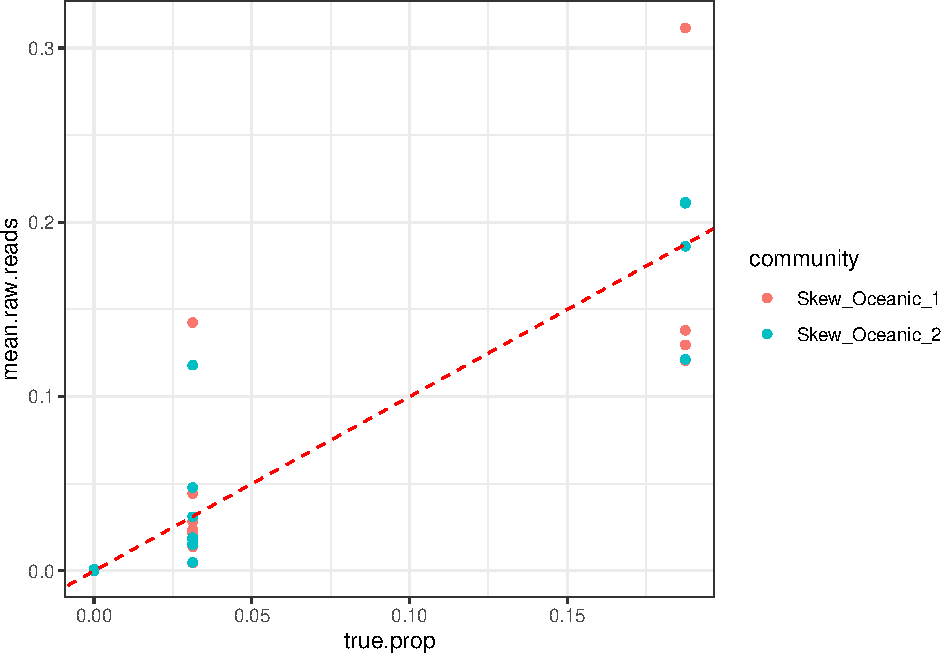
\includegraphics{Appendix-S4_files/figure-latex/stan_plots-1.pdf}

\begin{Shaded}
\begin{Highlighting}[]
\CommentTok{\# not so hot.}

\CommentTok{\# Better if you use point estimates from the model.}
\FunctionTok{ggplot}\NormalTok{(result.dat) }\SpecialCharTok{+}
    \FunctionTok{geom\_point}\NormalTok{(}\FunctionTok{aes}\NormalTok{(}\AttributeTok{x=}\NormalTok{true.prop,}\AttributeTok{y=}\NormalTok{mlEst,}\AttributeTok{color=}\NormalTok{community)) }\SpecialCharTok{+}
    \FunctionTok{geom\_abline}\NormalTok{(}\AttributeTok{intercept =} \DecValTok{0}\NormalTok{,}\AttributeTok{slope=}\DecValTok{1}\NormalTok{,}\AttributeTok{color=}\StringTok{"red"}\NormalTok{,}\AttributeTok{linetype=}\StringTok{"dashed"}\NormalTok{) }\SpecialCharTok{+}
    \FunctionTok{theme\_bw}\NormalTok{()}
\end{Highlighting}
\end{Shaded}

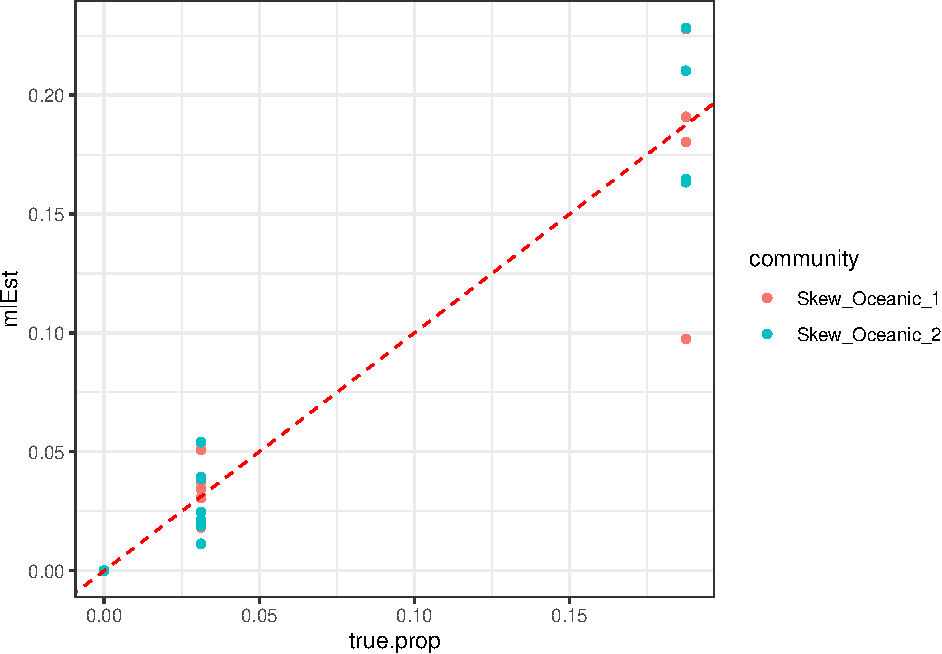
\includegraphics{Appendix-S4_files/figure-latex/stan_plots-2.pdf}

\begin{Shaded}
\begin{Highlighting}[]
\CommentTok{\# Or you can use the information from the draws to provide some uncertainty bounds.}
\CommentTok{\# Note that there are some mighty big error bars there.}
\FunctionTok{ggplot}\NormalTok{(result.dat) }\SpecialCharTok{+}
    \FunctionTok{geom\_point}\NormalTok{(}\FunctionTok{aes}\NormalTok{(}\AttributeTok{x=}\NormalTok{true.prop,}\AttributeTok{y=}\NormalTok{Mean,}\AttributeTok{color=}\NormalTok{community)) }\SpecialCharTok{+}
    \FunctionTok{geom\_errorbar}\NormalTok{(}\FunctionTok{aes}\NormalTok{(}\AttributeTok{x=}\NormalTok{true.prop,}\AttributeTok{ymin=}\NormalTok{q0}\FloatTok{.05}\NormalTok{,}\AttributeTok{ymax=}\NormalTok{q0}\FloatTok{.95}\NormalTok{,Mean,}\AttributeTok{color=}\NormalTok{community),}\AttributeTok{alpha=}\FloatTok{0.5}\NormalTok{,}\AttributeTok{width=}\DecValTok{0}\NormalTok{) }\SpecialCharTok{+}
    \FunctionTok{geom\_abline}\NormalTok{(}\AttributeTok{intercept =} \DecValTok{0}\NormalTok{,}\AttributeTok{slope=}\DecValTok{1}\NormalTok{,}\AttributeTok{color=}\StringTok{"red"}\NormalTok{,}\AttributeTok{linetype=}\StringTok{"dashed"}\NormalTok{) }\SpecialCharTok{+}
    \FunctionTok{theme\_bw}\NormalTok{()}
\end{Highlighting}
\end{Shaded}

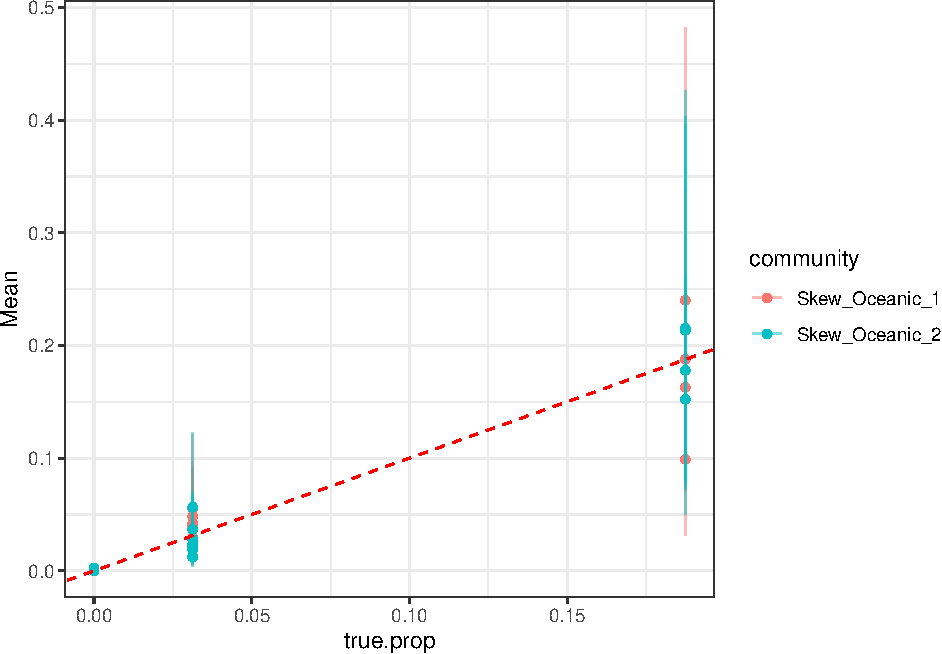
\includegraphics{Appendix-S4_files/figure-latex/stan_plots-3.pdf}

\begin{Shaded}
\begin{Highlighting}[]
\CommentTok{\# note that the estimates from the maximum likelihood and the draws are close by not identical.}
\FunctionTok{ggplot}\NormalTok{(result.dat) }\SpecialCharTok{+}
    \FunctionTok{geom\_point}\NormalTok{(}\FunctionTok{aes}\NormalTok{(}\AttributeTok{x=}\NormalTok{mlEst,}\AttributeTok{y=}\NormalTok{Mean,}\AttributeTok{color=}\NormalTok{community)) }\SpecialCharTok{+}
    \FunctionTok{geom\_abline}\NormalTok{(}\AttributeTok{intercept =} \DecValTok{0}\NormalTok{,}\AttributeTok{slope=}\DecValTok{1}\NormalTok{,}\AttributeTok{color=}\StringTok{"red"}\NormalTok{,}\AttributeTok{linetype=}\StringTok{"dashed"}\NormalTok{) }\SpecialCharTok{+}
    \FunctionTok{theme\_bw}\NormalTok{()}
\end{Highlighting}
\end{Shaded}

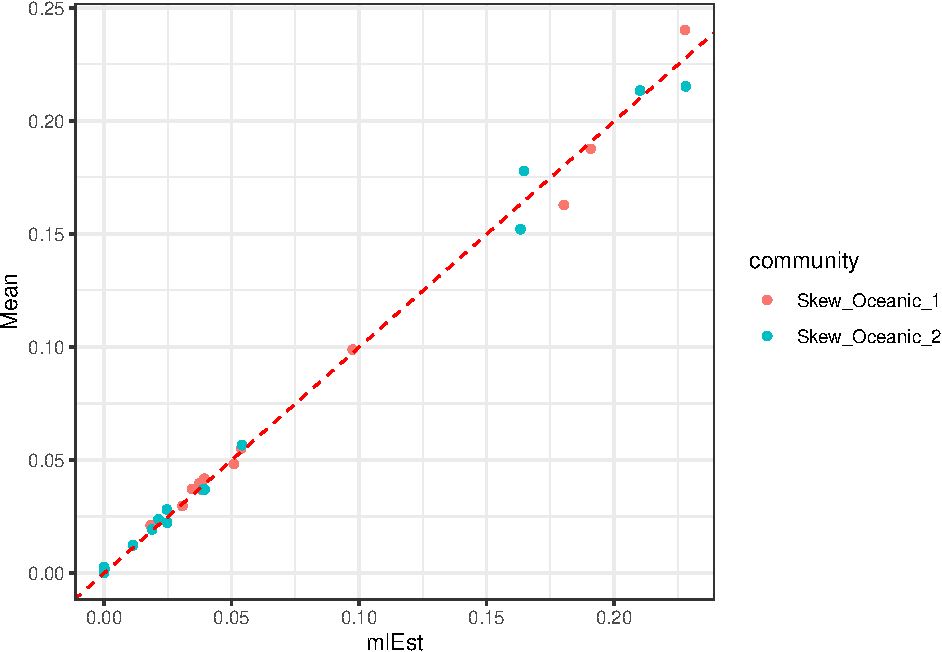
\includegraphics{Appendix-S4_files/figure-latex/stan_plots-4.pdf}

\hypertarget{bayesian-version}{%
\subsection{Bayesian version}\label{bayesian-version}}

OK. This is the full Bayesian version. On my computer it takes a minute
or two. I have commented out the actual estimation and included
summarized output as a

\begin{Shaded}
\begin{Highlighting}[]
  \DocumentationTok{\#\#\#\#\#\#\#\#\#\#\#\#\#\#\#\#\#\#\#\#\#\#\#\#\#\#\#\#\#\#\#\#\#\#\#\#\#\#\#\#\#}
\CommentTok{\#Bayesian Estimation}
\CommentTok{\# This is a very small problem so this runs pretty quick.}
\NormalTok{N\_CHAIN }\OtherTok{=} \DecValTok{3}
\NormalTok{Warm }\OtherTok{=} \DecValTok{500}
\NormalTok{Iter }\OtherTok{=} \DecValTok{1000}
\NormalTok{Treedepth }\OtherTok{=} \DecValTok{13}
\NormalTok{Adapt\_delta }\OtherTok{=} \FloatTok{0.8}

\CommentTok{\# This is the code to actually run the model.  It is commented out for speed}

\CommentTok{\# rstan\_options(auto\_write = TRUE)}
\CommentTok{\# options(mc.cores = parallel::detectCores())}
\CommentTok{\# \# you may have to specify a correct path for this to work...}
\CommentTok{\# stanMod = stan(file = "quant\_metabar\_multinom.stan" ,data = stan\_data,}
\CommentTok{\#                verbose = FALSE, chains = N\_CHAIN, thin = 1,}
\CommentTok{\#                warmup = Warm, iter = Warm + Iter,}
\CommentTok{\#                control = list(adapt\_init\_buffer = 175,}
\CommentTok{\#                               max\_treedepth=Treedepth,}
\CommentTok{\#                               stepsize=0.01,}
\CommentTok{\#                               adapt\_delta=Adapt\_delta,}
\CommentTok{\#                               metric="diag\_e"),}
\CommentTok{\#                pars = stan\_pars,}
\CommentTok{\#                \#refresh = 10,}
\CommentTok{\#                boost\_lib = NULL,}
\CommentTok{\#                init = stan\_init\_f2(n.chain=N\_CHAIN,N\_species=N\_species)}
\CommentTok{\#                \#sample\_file = paste0("./tmpF.csv")}
\CommentTok{\# )}
\CommentTok{\# }
\CommentTok{\# pars \textless{}{-} rstan::extract(stanMod, permuted = TRUE)}
\CommentTok{\# samp\_params \textless{}{-} get\_sampler\_params(stanMod)}
\CommentTok{\# }
\CommentTok{\# stanMod\_summary \textless{}{-} list()}
\CommentTok{\# stanMod\_summary[["alpha"]] \textless{}{-} summary(stanMod,pars="alpha")$summary}
\CommentTok{\# stanMod\_summary[["tau"]] \textless{}{-} summary(stanMod,pars=c("tau"))$summary}
\CommentTok{\# stanMod\_summary[["beta"]] \textless{}{-} summary(stanMod,pars="beta")$summary}
\CommentTok{\# stanMod\_summary[["eta\_samp\_raw"]] \textless{}{-} summary(stanMod,pars="eta\_samp")$summary}
\CommentTok{\# stanMod\_summary[["eta\_mock\_raw"]] \textless{}{-} summary(stanMod,pars="eta\_mock")$summary}
\CommentTok{\# stanMod\_summary[["mu\_samp"]] \textless{}{-} summary(stanMod,pars="mu\_samp")$summary}
\CommentTok{\# stanMod\_summary[["mu\_mock"]] \textless{}{-} summary(stanMod,pars="mu\_mock")$summary}
\CommentTok{\# stanMod\_summary[["int\_samp\_small"]] \textless{}{-} summary(stanMod,pars="int\_samp\_small")$summary}
\CommentTok{\# }
\CommentTok{\# Output \textless{}{-} list(}
\CommentTok{\# }
\CommentTok{\#   env = env,  \#environmental sample data}
\CommentTok{\#   mc = mc, \#mock data}
\CommentTok{\#   Species = unique(mc$Species),}
\CommentTok{\# }
\CommentTok{\#   \# Input data}
\CommentTok{\#   p\_true = p\_mock,}
\CommentTok{\#   p\_samp\_all = sample\_data,}
\CommentTok{\#   p\_mock\_all = mock\_data,}
\CommentTok{\# }
\CommentTok{\#   \# stan input objects}
\CommentTok{\#   stan\_data = stan\_data,}
\CommentTok{\#   Warm=Warm,}
\CommentTok{\#   Iter=Iter,}
\CommentTok{\# }
\CommentTok{\#   \# Fitted Objects}
\CommentTok{\#   stanMod = stanMod, \# Full stan Model fitted object}
\CommentTok{\#   pars = pars, \# MCMC output}
\CommentTok{\#   samp\_params=samp\_params, \# Sampler information}
\CommentTok{\#   stanMod\_summary = stanMod\_summary \# posterior summaries.}
\CommentTok{\# )}
\CommentTok{\# }
\CommentTok{\# \# This saves things to file so you don\textquotesingle{}t have to run the model every time.}
\CommentTok{\# save(Output,file=paste0("Fish\_Oceanic\_crossValidate",".Rdata"))}
\end{Highlighting}
\end{Shaded}

\begin{Shaded}
\begin{Highlighting}[]
\CommentTok{\# Extract estimates and make basic plots. }
\CommentTok{\# read in the file created in the previous chunk.}
\FunctionTok{load}\NormalTok{(}\StringTok{"Fish\_Oceanic\_crossValidate.Rdata"}\NormalTok{)}
\NormalTok{mock2 }\OtherTok{\textless{}{-}}\NormalTok{ Output }\CommentTok{\# This is the cross validation that uses only the 39 cycle even communities}

\DocumentationTok{\#\#\#\#\#\#\#\#\#\#\#\#\#\#\#\#\#\#\#\#\#\#\#\#\#\#\#\#\#\#\#\#\#\#\#\#\#\#\#\#\#\#\#\#\#\#\#\#\#\#\#\#\#\#\#\#\#}
\CommentTok{\# Mock2}
\DocumentationTok{\#\#\#\#\#\#\#\#\#\#\#\#\#\#\#\#\#\#\#\#\#\#\#\#\#\#\#\#\#\#\#\#\#\#\#\#\#\#\#\#\#\#\#\#\#\#\#\#\#\#\#\#\#\#\#\#\#}
\CommentTok{\# summarize raw estimates from reads for each species.}
\NormalTok{mock2.raw }\OtherTok{\textless{}{-}}\NormalTok{ mock2}\SpecialCharTok{$}\NormalTok{env }\SpecialCharTok{\%\textgreater{}\%} \FunctionTok{group\_by}\NormalTok{(community,Cycles,tech\_rep) }\SpecialCharTok{\%\textgreater{}\%}
  \FunctionTok{mutate}\NormalTok{(}\AttributeTok{sum.ng =} \FunctionTok{sum}\NormalTok{(start\_conc\_ng),}
         \AttributeTok{true.prop =}\NormalTok{ start\_conc\_ng }\SpecialCharTok{/}\NormalTok{ sum.ng) }\SpecialCharTok{\%\textgreater{}\%}
  \FunctionTok{ungroup}\NormalTok{() }\SpecialCharTok{\%\textgreater{}\%}
  \FunctionTok{group\_by}\NormalTok{(Species,community,Cycles,true.prop) }\SpecialCharTok{\%\textgreater{}\%}
  \FunctionTok{summarise}\NormalTok{(}\AttributeTok{simple.Mean=}\FunctionTok{mean}\NormalTok{(propReads),}
            \AttributeTok{simple.N =} \FunctionTok{length}\NormalTok{(tech\_rep)) }\SpecialCharTok{\%\textgreater{}\%}
  \FunctionTok{replace\_na}\NormalTok{(}\FunctionTok{list}\NormalTok{(}\AttributeTok{raw.Mean=}\DecValTok{0}\NormalTok{,}\AttributeTok{raw.SD=}\DecValTok{0}\NormalTok{,}\AttributeTok{raw.SE=}\DecValTok{0}\NormalTok{))}

\CommentTok{\# extract predicted proportions from the posterior}
\NormalTok{COM }\OtherTok{\textless{}{-}} \FunctionTok{data.frame}\NormalTok{(}\AttributeTok{community =} \FunctionTok{levels}\NormalTok{(mock2}\SpecialCharTok{$}\NormalTok{env}\SpecialCharTok{$}\NormalTok{community }\SpecialCharTok{\%\textgreater{}\%} \FunctionTok{as.factor}\NormalTok{()))}
\NormalTok{COM}\SpecialCharTok{$}\NormalTok{comm\_idx }\OtherTok{\textless{}{-}} \DecValTok{1}\SpecialCharTok{:}\FunctionTok{nrow}\NormalTok{(COM)}
\NormalTok{SP  }\OtherTok{\textless{}{-}}\NormalTok{ mock2}\SpecialCharTok{$}\NormalTok{env }\SpecialCharTok{\%\textgreater{}\%} \FunctionTok{distinct}\NormalTok{(Species,sp\_idx) }\SpecialCharTok{\%\textgreater{}\%} \FunctionTok{as.data.frame}\NormalTok{()}

\CommentTok{\# These are the predicted intercepts for the posteriors}
\NormalTok{beta\_posterior }\OtherTok{\textless{}{-}}\NormalTok{ mock2}\SpecialCharTok{$}\NormalTok{stanMod\_summary[[}\StringTok{"int\_samp\_small"}\NormalTok{]][, }\FunctionTok{c}\NormalTok{(}\DecValTok{1}\NormalTok{,}\DecValTok{4}\SpecialCharTok{:}\DecValTok{8}\NormalTok{)]}
\FunctionTok{colnames}\NormalTok{(beta\_posterior) }\OtherTok{\textless{}{-}} \FunctionTok{paste0}\NormalTok{(}\StringTok{"mock2."}\NormalTok{,}\FunctionTok{substr}\NormalTok{(}\FunctionTok{colnames}\NormalTok{(beta\_posterior),}\DecValTok{1}\NormalTok{,}\FunctionTok{nchar}\NormalTok{(}\FunctionTok{colnames}\NormalTok{(beta\_posterior))}\SpecialCharTok{{-}}\DecValTok{1}\NormalTok{))}
\FunctionTok{colnames}\NormalTok{(beta\_posterior)[}\DecValTok{1}\NormalTok{] }\OtherTok{\textless{}{-}} \StringTok{"mock2.mean"}
\NormalTok{beta\_posterior }\OtherTok{\textless{}{-}} \FunctionTok{as.data.frame}\NormalTok{(beta\_posterior)}

\NormalTok{mock2.post }\OtherTok{\textless{}{-}}\FunctionTok{expand.grid}\NormalTok{(}\AttributeTok{comm\_idx =}\NormalTok{ COM}\SpecialCharTok{$}\NormalTok{comm\_idx,}\AttributeTok{sp\_idx =}\NormalTok{SP}\SpecialCharTok{$}\NormalTok{sp\_idx) }\SpecialCharTok{\%\textgreater{}\%} 
  \FunctionTok{arrange}\NormalTok{(comm\_idx,sp\_idx) }\SpecialCharTok{\%\textgreater{}\%} 
  \FunctionTok{left\_join}\NormalTok{(.,COM) }\SpecialCharTok{\%\textgreater{}\%} 
  \FunctionTok{left\_join}\NormalTok{(.,SP) }\SpecialCharTok{\%\textgreater{}\%} 
  \FunctionTok{bind\_cols}\NormalTok{(.,beta\_posterior)}

\CommentTok{\# Combine the raw estimates and posterior estimates}
\NormalTok{mock2.all }\OtherTok{\textless{}{-}} \FunctionTok{full\_join}\NormalTok{(mock2.raw,mock2.post)}

\NormalTok{mock2.all }\OtherTok{\textless{}{-}}\NormalTok{ mock2.all }\SpecialCharTok{\%\textgreater{}\%} \FunctionTok{mutate}\NormalTok{(}\AttributeTok{true.cat=} \FunctionTok{ifelse}\NormalTok{(true.prop}\SpecialCharTok{\textgreater{}}\FloatTok{0.1}\NormalTok{,}\StringTok{"big"}\NormalTok{,}\StringTok{"small"}\NormalTok{))}

\CommentTok{\# pull out just ocean.skew.dat for plotting.}
\NormalTok{spread}\OtherTok{=}\FloatTok{0.15}
\NormalTok{ocean.skew1.dat }\OtherTok{\textless{}{-}}\NormalTok{ mock2.all }\SpecialCharTok{\%\textgreater{}\%} 
  \FunctionTok{filter}\NormalTok{(true.prop }\SpecialCharTok{\textgreater{}} \DecValTok{0}\NormalTok{,community}\SpecialCharTok{==}\StringTok{"Skew\_Oceanic\_1"}\NormalTok{)}
\NormalTok{ocean.skew1.dat }\OtherTok{\textless{}{-}} \FunctionTok{bind\_cols}\NormalTok{(ocean.skew1.dat, }
                             \FunctionTok{data.frame}\NormalTok{(}\AttributeTok{offset=}     \FunctionTok{seq}\NormalTok{(}\SpecialCharTok{{-}}\NormalTok{spread,spread,}\AttributeTok{length.out=}\FunctionTok{nrow}\NormalTok{(ocean.skew1.dat))))}

\NormalTok{ocean.skew2.dat }\OtherTok{\textless{}{-}}\NormalTok{ mock2.all }\SpecialCharTok{\%\textgreater{}\%} 
  \FunctionTok{filter}\NormalTok{(true.prop }\SpecialCharTok{\textgreater{}} \DecValTok{0}\NormalTok{,community}\SpecialCharTok{==}\StringTok{"Skew\_Oceanic\_2"}\NormalTok{)}
\NormalTok{ocean.skew2.dat }\OtherTok{\textless{}{-}} \FunctionTok{bind\_cols}\NormalTok{(ocean.skew2.dat, }
                            \FunctionTok{data.frame}\NormalTok{(}\AttributeTok{offset=} \FunctionTok{seq}\NormalTok{(}\SpecialCharTok{{-}}\NormalTok{spread,spread,}\AttributeTok{length.out=}\FunctionTok{nrow}\NormalTok{(ocean.skew2.dat))))}

\CommentTok{\# Make plots}
\NormalTok{BREAKS }\OtherTok{\textless{}{-}} \FunctionTok{c}\NormalTok{(}\FloatTok{0.0}\NormalTok{,}\FloatTok{0.01}\NormalTok{,}\FloatTok{0.05}\NormalTok{,}\FloatTok{0.10}\NormalTok{,}\FloatTok{0.20}\NormalTok{,}\FloatTok{0.30}\NormalTok{,}\FloatTok{0.40}\NormalTok{,}\FloatTok{0.6}\NormalTok{,}\FloatTok{0.8}\NormalTok{)}
\NormalTok{x.labs }\OtherTok{\textless{}{-}} \FunctionTok{c}\NormalTok{(}\StringTok{"Raw reads"}\NormalTok{,}\StringTok{"Mock"}\NormalTok{)}
\NormalTok{x.at   }\OtherTok{\textless{}{-}} \FunctionTok{c}\NormalTok{(}\DecValTok{1}\NormalTok{,}\DecValTok{2}\NormalTok{)}

\NormalTok{skew\_plot }\OtherTok{\textless{}{-}} \ControlFlowTok{function}\NormalTok{(dat,}
                      \AttributeTok{BREAKS=}\NormalTok{BREAKS,}\AttributeTok{x.labs=}\NormalTok{x.labs,}\AttributeTok{x.at=}\NormalTok{x.at)\{}
  
\NormalTok{    shape.val }\OtherTok{=} \FunctionTok{c}\NormalTok{(}\DecValTok{21}\NormalTok{,}\DecValTok{22}\NormalTok{)}
\NormalTok{    col.val }\OtherTok{=} \FunctionTok{pal\_jco}\NormalTok{(}\AttributeTok{palette =} \FunctionTok{c}\NormalTok{(}\StringTok{"default"}\NormalTok{), }\AttributeTok{alpha =} \DecValTok{1}\NormalTok{)(}\DecValTok{10}\NormalTok{)[}\FunctionTok{c}\NormalTok{(}\DecValTok{1}\NormalTok{,}\DecValTok{4}\NormalTok{)]}
  
\NormalTok{  skew.plot }\OtherTok{\textless{}{-}}  \FunctionTok{ggplot}\NormalTok{(dat) }\SpecialCharTok{+}
    \FunctionTok{geom\_point}\NormalTok{(}\FunctionTok{aes}\NormalTok{(}\AttributeTok{x=}\DecValTok{1}\SpecialCharTok{+}\NormalTok{offset,}\AttributeTok{y=}\NormalTok{simple.Mean,}\AttributeTok{shape=}\NormalTok{true.cat,}\AttributeTok{fill=}\NormalTok{true.cat,}\AttributeTok{color=}\NormalTok{true.cat),}\AttributeTok{size=}\DecValTok{2}\NormalTok{) }\SpecialCharTok{+}
    \FunctionTok{geom\_errorbar}\NormalTok{(}\FunctionTok{aes}\NormalTok{(}\AttributeTok{x=}\DecValTok{2}\SpecialCharTok{+}\NormalTok{offset,}
                      \AttributeTok{ymin=}\NormalTok{ mock2.}\FloatTok{2.5}\NormalTok{, }
                      \AttributeTok{ymax=}\NormalTok{ mock2.}\FloatTok{97.5}\NormalTok{,}\AttributeTok{color=}\NormalTok{true.cat),}\AttributeTok{width=}\DecValTok{0}\NormalTok{,}\AttributeTok{alpha=}\FloatTok{0.75}\NormalTok{)   }\SpecialCharTok{+}
    \FunctionTok{geom\_point}\NormalTok{(}\FunctionTok{aes}\NormalTok{(}\AttributeTok{x=}\DecValTok{2}\SpecialCharTok{+}\NormalTok{offset,mock2.mean,}\AttributeTok{shape=}\NormalTok{true.cat,}\AttributeTok{fill=}\NormalTok{true.cat,}\AttributeTok{color=}\NormalTok{true.cat),}\AttributeTok{size=}\DecValTok{2}\NormalTok{) }\SpecialCharTok{+}
    \FunctionTok{scale\_shape\_manual}\NormalTok{(}\AttributeTok{values =}\FunctionTok{c}\NormalTok{(}\DecValTok{21}\NormalTok{,}\DecValTok{22}\NormalTok{)) }\SpecialCharTok{+}
    \FunctionTok{scale\_fill\_manual}\NormalTok{(}\AttributeTok{values=}\NormalTok{ col.val, }\StringTok{"True value"}\NormalTok{) }\SpecialCharTok{+}
    \FunctionTok{scale\_color\_manual}\NormalTok{(}\AttributeTok{values=}\NormalTok{ col.val,}\StringTok{"True value"}\NormalTok{) }\SpecialCharTok{+}
    \FunctionTok{scale\_y\_continuous}\NormalTok{(}\StringTok{"Proportion"}\NormalTok{,}
                       \AttributeTok{trans=}\StringTok{"sqrt"}\NormalTok{,}
                       \CommentTok{\# trans="log",}
                       \AttributeTok{breaks =}\NormalTok{ BREAKS,}\AttributeTok{expand=}\FunctionTok{c}\NormalTok{(}\DecValTok{0}\NormalTok{,}\ConstantTok{NA}\NormalTok{),}\AttributeTok{limits =} \FunctionTok{c}\NormalTok{(}\DecValTok{0}\NormalTok{,}\ConstantTok{NA}\NormalTok{)) }\SpecialCharTok{+}
    \FunctionTok{geom\_hline}\NormalTok{(}\FunctionTok{aes}\NormalTok{(}\AttributeTok{yintercept =}\NormalTok{ true.prop,}\AttributeTok{color=}\NormalTok{true.cat),}\AttributeTok{linetype=}\StringTok{"dashed"}\NormalTok{) }\SpecialCharTok{+}
    \CommentTok{\#geom\_point(aes(x=0.70,y=true.prop,shape=true.cat,fill=true.cat),size=3) +}
    \FunctionTok{scale\_x\_continuous}\NormalTok{(}\AttributeTok{name=}\ConstantTok{NULL}\NormalTok{,}\AttributeTok{breaks=}\NormalTok{x.at,}\AttributeTok{labels =}\NormalTok{ x.labs) }\SpecialCharTok{+}
    \FunctionTok{theme\_classic}\NormalTok{() }\SpecialCharTok{+}
    \FunctionTok{theme}\NormalTok{(}\AttributeTok{legend.position =} \StringTok{"none"}\NormalTok{)}
  
  \FunctionTok{return}\NormalTok{(skew.plot)}
\NormalTok{\}}


\NormalTok{ocean.skew}\FloatTok{.1} \OtherTok{\textless{}{-}} \FunctionTok{skew\_plot}\NormalTok{(}\AttributeTok{dat=}\NormalTok{ocean.skew1.dat,}
                          \AttributeTok{BREAKS=}\NormalTok{BREAKS,}\AttributeTok{x.labs=}\NormalTok{x.labs,}\AttributeTok{x.at=}\NormalTok{x.at) }
\FunctionTok{print}\NormalTok{(ocean.skew}\FloatTok{.1}  \SpecialCharTok{+}\FunctionTok{ggtitle}\NormalTok{(}\StringTok{"Ocean skew 1"}\NormalTok{))                }
\end{Highlighting}
\end{Shaded}

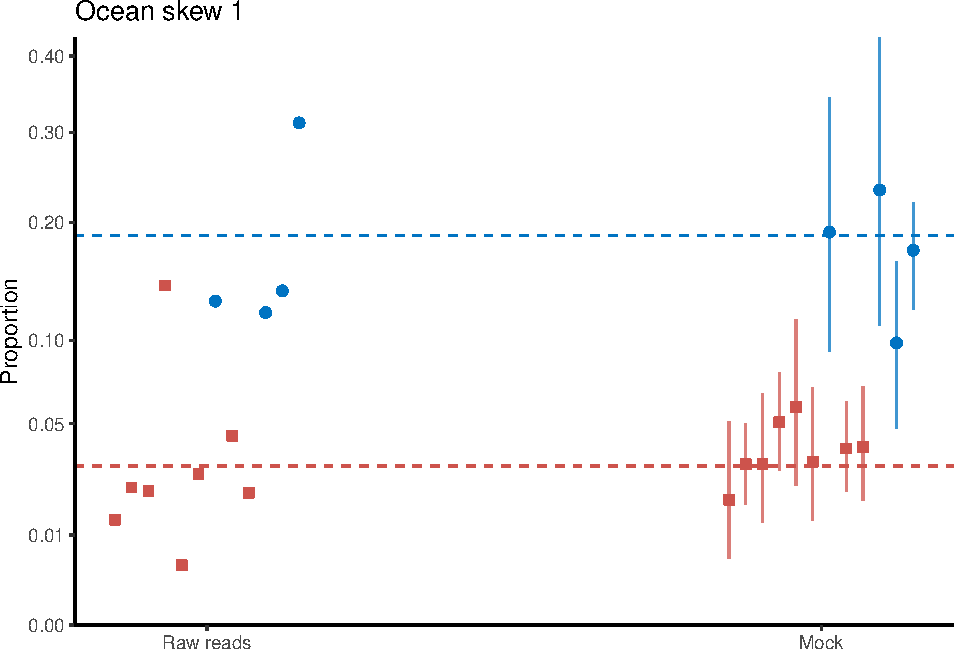
\includegraphics{Appendix-S4_files/figure-latex/stan_plotting_bayes-1.pdf}

\begin{Shaded}
\begin{Highlighting}[]
\NormalTok{ocean.skew}\FloatTok{.2} \OtherTok{\textless{}{-}} \FunctionTok{skew\_plot}\NormalTok{(}\AttributeTok{dat=}\NormalTok{ocean.skew2.dat,}
                          \AttributeTok{BREAKS=}\NormalTok{BREAKS,}\AttributeTok{x.labs=}\NormalTok{x.labs,}\AttributeTok{x.at=}\NormalTok{x.at) }
\FunctionTok{print}\NormalTok{(ocean.skew}\FloatTok{.2} \SpecialCharTok{+}\FunctionTok{ggtitle}\NormalTok{(}\StringTok{"Ocean skew 2"}\NormalTok{))}
\end{Highlighting}
\end{Shaded}

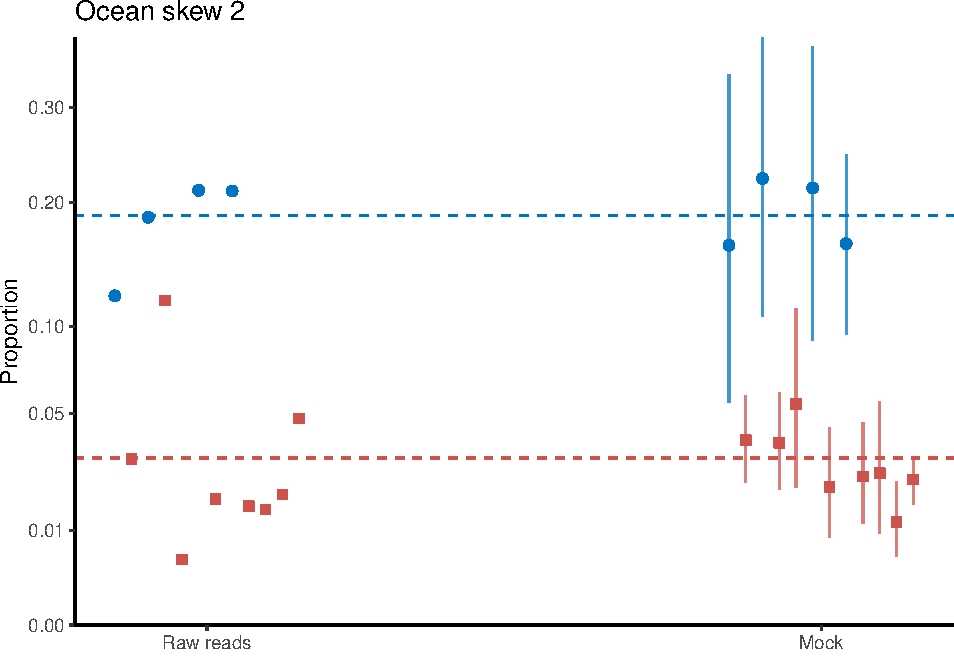
\includegraphics{Appendix-S4_files/figure-latex/stan_plotting_bayes-2.pdf}

\hypertarget{other-versions}{%
\subsection{Other versions}\label{other-versions}}

OK. The above is for a model with technical replicates. If you don't
have technical replication, you can't estimate some of the parameters. A
simplified model version for that scenario involves using the file
\emph{quant\_metabar\_no\_overdispersion.stan}. You would change the
required stan model files like so:

\begin{Shaded}
\begin{Highlighting}[]
\CommentTok{\# These are the parameters that are to be monitored during optimization or MCMC:}
\NormalTok{stan\_pars }\OtherTok{\textless{}{-}} \FunctionTok{c}\NormalTok{(}
  \StringTok{"alpha"}\NormalTok{, }\CommentTok{\# efficiencies relative to the reference species}
  \StringTok{"beta"}\NormalTok{,  }\CommentTok{\# parameters for each site (NOT )}
  \StringTok{"mu\_samp"}\NormalTok{, }\CommentTok{\# Predicted proportions for each species{-}site (unknown samples)}
  \StringTok{"mu\_mock"}\NormalTok{, }\CommentTok{\# Predicted proportions for each species{-}site (mock samples)}
  \StringTok{"int\_samp\_small"} \CommentTok{\# this is the predicted intercept for each site }
\NormalTok{)}
\end{Highlighting}
\end{Shaded}

and everything else can be used as above. Essentially, you can't
estimate the random effects that allow for over-dispersion with a single
replicate. If you have a mix of replication and no replication, that is
trickier but we can likely work something out if you want to work on
that.

There are two other files that might be of interest that allow you to
fit an equivalent model assuming no amplification differences among
species. These are:

\emph{quant\_metabar\_no\_mock\_no\_alpha.stan}

which allows you to fit a model with over-dispersion in the observations
and

\emph{quant\_metabar\_no\_overdispersion\_no\_alpha.stan}

which does not allow for over-dispersion.

\end{document}
